 %%%%Textart%%%%
\documentclass[a4paper, 12pt, oneside, BCOR=0cm]{scrbook}

%Alle packages, commands, etc ausgelagert in mystyle.sty
\usepackage{mystyle}



\begin{document}
\begin{titlepage}
\begin{center}
    \Large\textbf{Department of Physics and Astronomy\\Ruprecht Karl University of Heidelberg}
    
    \vfill
    
    \large
    Bachelor Thesis in Physics\\
    submitted by\\
    \vspace{0.5cm}
    \Large\textbf{Tim Küchler}\\
    \normalsize
    \vspace{0.5cm}
    born in Heidelberg (Germany)\\
    \vspace{0.5cm}
    \Large\textbf{2021}
    \normalsize
    \afterpage{\blankpage}
    \newpage
    \thispagestyle{empty}
    \Large\textbf{Semantic Image Synthesis with Score-Based Generative Models}
    
    \vfill
    
    \large
    This Bachelor Thesis has been carried out by Tim Küchler\\
    at the\\
    Heidelberg Collaboratory for Image Processing\\
    and the\\
    Interdisciplinary Center for Scientific Computing\\
    under the supervision of\\
    Prof. Dr. Björn Ommer and $\dots$
    \afterpage{\blankpage}
\end{center}
\end{titlepage}
%
\frontmatter

\chapter*{Acknowledgements}
\thispagestyle{empty}
%This thesis is the grand finale of a three-year adventure with many ups and downs. But you can't go through an adventure like this alone. It takes emotional support, competent advice and a lot of great moments of togetherness to finally reach the destination on such a journey. And finally being able to say: You have made it!
\\

\noindent I thank my family, my friends and everyone else who believed in me and was there for me when I needed them. Moreover, I thank all persons who did not get the attention they deserved during this time and yet were patient with me. At the end of the day, I can only say one thing:
\begin{center}
    \textbf{Without you all, this adventure would have been a different one!}
\end{center}
\afterpage{\blankpage}

\chapter*{Abstract}
\noindent\textbf{Semantische Bildsynthese mit Score-basierten, generativen Modellen:}\\[0.3cm]
\noindent Die künstliche Bilderzeugung ist ein zukunftsweisendes Forschungsgebiet der modernen Informatik. Wenn die semantische Bildinformation des generierten Bildes beeinflusst werden soll oder die vorgesehene Aufgabe eine pixelweise Kontrolle über das Ergebnis erfordert, wird semantische Bildsynthese benötigt. In dieser Arbeit zeigen wir einen Ansatz, der das neue und vielversprechende Konzept der Score-basierten generativen Modelle für die semantische Bildsynthese verwendet. Dazu trainieren wir zunächst ein rauschbedingtes Score-Netz auf einem Datensatz, das dann mit einem sorgfältig entworfenen rauschbedingten semantischen Segmentierungsnetz kombiniert wird, welches auf demselben Datensatz trainiert wurde. Anschließend vergleichen wir unsere Ergebnisse auf dem Cityscapes-Datensatz \cite{cityscapes} quantitativ mit State-of-the-Art-Modellen wie CRN \cite{crn}, pix2pixHD \cite{pix2pixHD} und SPADE \cite{spade} unter Verwendung der FID-Scores sowie der Pixelgenauigkeit und der mittleren IoU. Darüber hinaus generieren wir hochauflösende Landschaftsbilder unter Verwendung von Bildern, die wir von der Bildplatform Flickr gesammelt haben. Abschließend zeigen wir die Grenzen unseres Ansatzes am ADE20K-Datensatz \cite{ade20k} und weisen auf Herausforderungen hin, deren Lösung in der zukünftigen Forschung die semantische Bildsynthese mit Score-basierten generativen Modellen zu einem leistungsfähigen, vielseitigen und einfach zu verwendenden Framework machen könnte.\\[0.3cm]
\noindent\textbf{Semantic Image Synthesis with Score-Based Generative Models:}\\[0.3cm]
\noindent Artificial image generation is a cutting-edge field of research in modern computer science. If the semantic image information of the generated image is to be influenced or the envised task requires pixel-wise control over the result, semantic image synthesis is needed. In this thesis, we show an approach using the new and promising concept of score-based generative models for semantic image synthesis. For this, we first train a noise-conditional score-network on the dataset, which is then combined with a carefully designed noise-conditional semantic segmentation network trained on the same dataset. We then quantitatively compare our results on the Cityscapes dataset \cite{cityscapes} with state-of-the-art models like CRN \cite{crn}, pix2pixHD \cite{pix2pixHD} and SPADE \cite{spade} using FID scores as well as pixel accuracy and mean IoU. Furthermore, we generate high resolution landscape images using images scraped from Flickr. Finally, we show the limitations of our approach on the ADE20K dataset \cite{ade20k} and point out challenges whose solution in future research could make semantic image synthesis with score-based generative models a powerful, versatile and easy-to-use framework.
\thispagestyle{empty}
\afterpage{\blankpage}

\setcounter{tocdepth}{1}
\tableofcontents
\thispagestyle{empty}
\addtocontents{toc}{\protect\thispagestyle{empty}}
\afterpage{\blankpage}



\mainmatter
\chapter{Introduction}

\section{Generating data} \label{sec:1.1}
\thispagestyle{plain}
We as humans have been born as intelligent living beings. We use this intelligence to create things of indescribable creativity and complexity. All the more understandable is the drive to understand this creative process and to reproduce it artificially. And it is this drive that gave rise to a new branch of research in computer sciences, which finally led to the concept of \textit{Generative Modeling}.

\thispagestyle{plain}
Generative Modeling is an umbrella term describing artificial approaches to generate realistic data. The current state-of-the-art approaches are dominated by so called \textit{Deep Neural Networks}, complex artificial constructs which are partially inspired by the human brain. These networks are implemented as a computer program, using modern machine learning libraries such as \textit{PyTorch} \cite{pytorch} or \textit{TensorFlow} \cite{tensorflow}.

%
\begin{figure}[] \label{fig:1.1}
    \centering
    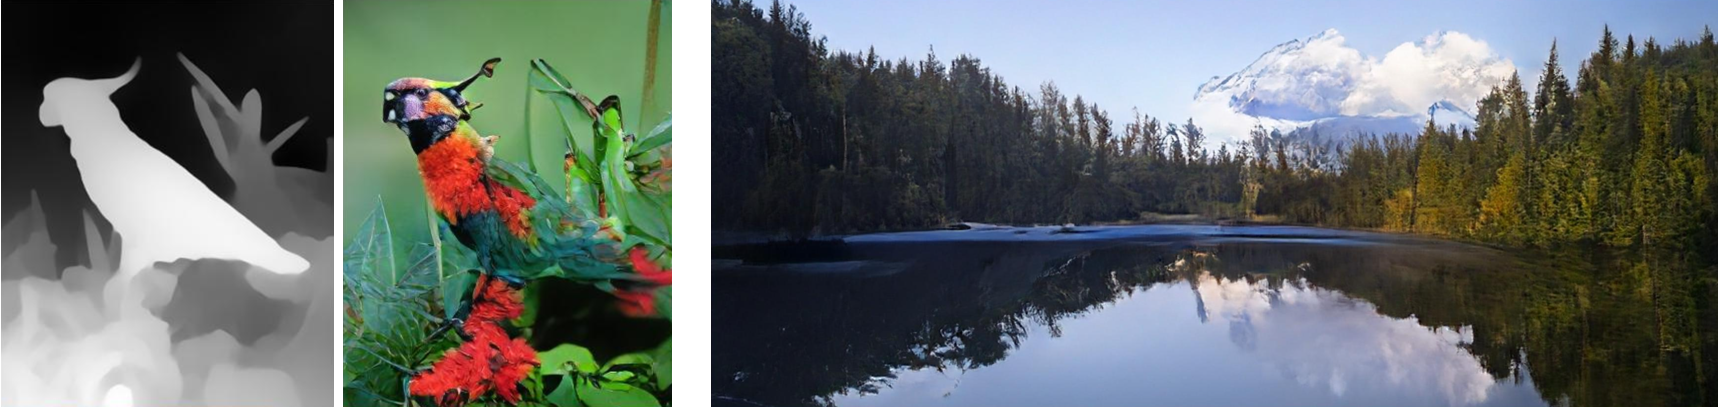
\includegraphics[width=0.8\textwidth]{Chapters/figures/transformer.PNG}
    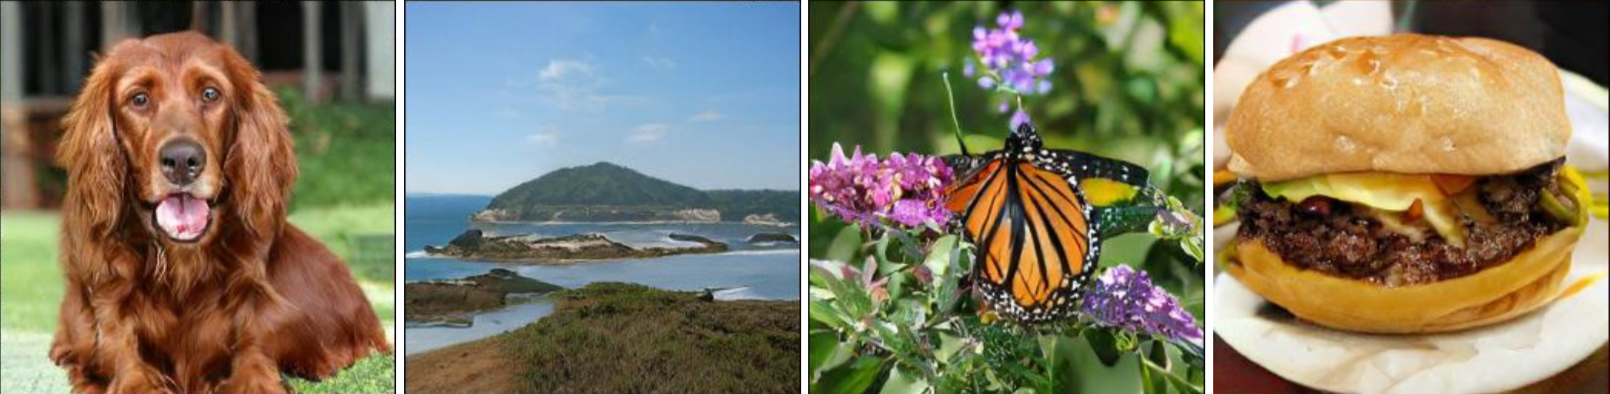
\includegraphics[width=0.8\textwidth]{Chapters/figures/biggan.PNG}
    \caption[Examples for state-of-the-art samples]{\textit{Top Left}: Depth-to-Image, \textit{Top Right}: Semantic synthesis, Images from \cite{taming}\\\textit{Bottom}: Class-conditional samples, Images from \cite{biggan}} 
\end{figure}
%
\thispagestyle{plain}
In the last years generative modeling has seen an \textbf{immense} progress in generating the most diverse types of data. Some results have even reached such a quality that they can hardly be distinguished from realistic data for the human eye (see e.g. \hyperref[fig:1.1]{Fig.\,1.1}). Some fields of generative modeling on which outstanding results have been achieved include image generation, video generation and audio and speech generation. In addition to the general push for better generation models, some models are already indispensable for various application purposes such as image processing, anomaly detection in medical context and generation of new data for scientific uses, e.g. the artificial generation of promising molecular candidates for the development of new effective drugs \cite{molgrad}.
\thispagestyle{plain}
%%%%%%%%%%%%%%%%%%%%%%%%%%%%%%%%%%%%%%%%%%%%%%%%%%%%%%%%%%%%%%%%%%%%%%%%%%%%%%%%%%%%%%%%%%%%
\section{Score-Based Generative Models - The new contenders to GANs?} 
\thispagestyle{plain}
"Creating noise from data is easy; creating data from noise is generative modeling" \cite{score_3}. This quote describes the operating principle of a novel model for generating data (\hyperref[sec:1.1]{Sec.\,1.1}), which we will explore in various ways in this paper.

The so-called \textit{Score-Based Generative Models} (SGMs) were recently proposed by Yang Song and Stefano Ermon \cite{score_1} in late 2020. As a generative model SGMs can be used to generate all kinds of data such as images, audio and graphs and they are capable of performing a variety of special tasks such as inpainting, colorization and image-to-image translation. As shown in outstanding results from recent work \cite{score_3} they are capable to keep up with state-of-the-art generative models such as Generative Adversarial Networks (GANs) \cite{gan_original} and Variational Autoencoders (VAEs) \cite{vae_original}. Therefore, SGMs have gained great attention in the scientific community and are already considered by some to be the "new contenders to GANs" \cite{blog}.

\thispagestyle{plain}
Score-Based Generative Models work by estimating the score of a given data distribution via score matching \cite{score_matching_original}. Because the score estimating technique is unstable or ill-defined for a real data distribution the initial images are perturbed by Gaussian noise. Starting from random noise, SGMs are able to generate completely new data.

\thispagestyle{plain}
%
\begin{figure}[]
    \centering
    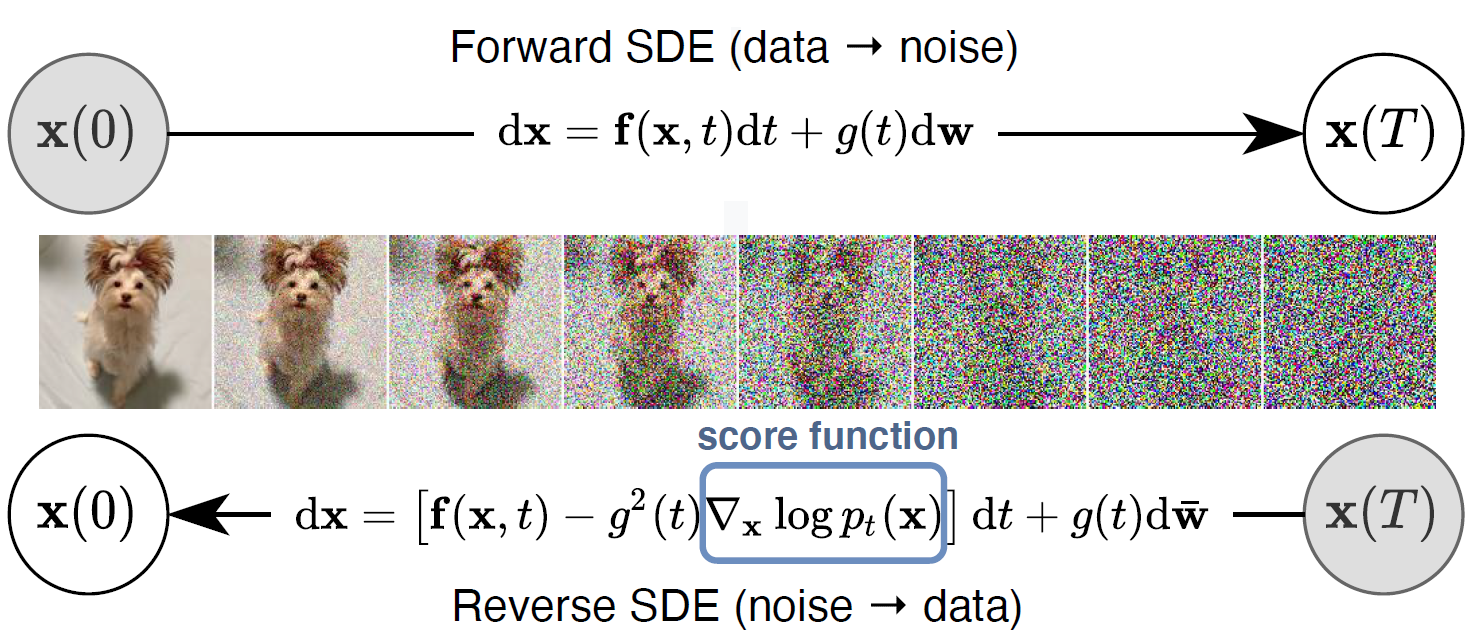
\includegraphics[width=0.8\textwidth]{Chapters/figures/sgm.PNG}
    \caption[The idea of Score-Based Generative Models]{The idea of SGMs: First the data distribution is perturbed via a diffusion process governed by a SDE. The scores of the noise distributions are learned by the score model and are then used to solve a reverse SDE to generate new data from noise. Figure from \cite{score_3}}
\end{figure}
%

\thispagestyle{plain}
SGMs have several advantages to other popular models. They do not rely on adversarial training, which is often unstable, they do not need a special architecture in order to be tractable, they do not need sampling during training and they can be used for different tasks such as inpainting, class-conditional generation and colorization without the need to retrain the model. Although SGMs are very slow in sampling, they have the advantage that there is an arbitrary possibility of combinations of sampling techniques and model architectures, allowing the search for a best-possible sampling procedure. All in all, these properties, together with the high quality of the recent results, make SGMs a promising new model for generative modeling.
%%%%%%%%%%%%%%%%%%%%%%%%%%%%%%%%%%%%%%%%%%%%%%%%%%%%%%%%%%%%%%%%%%%%%%%%%%%%%%%%%%%%%%%%%%%%%%%
\section{Semantic Segmentation and Semantic Synthesis} 
\thispagestyle{plain}
%
\begin{figure}[h!]
    \centering
    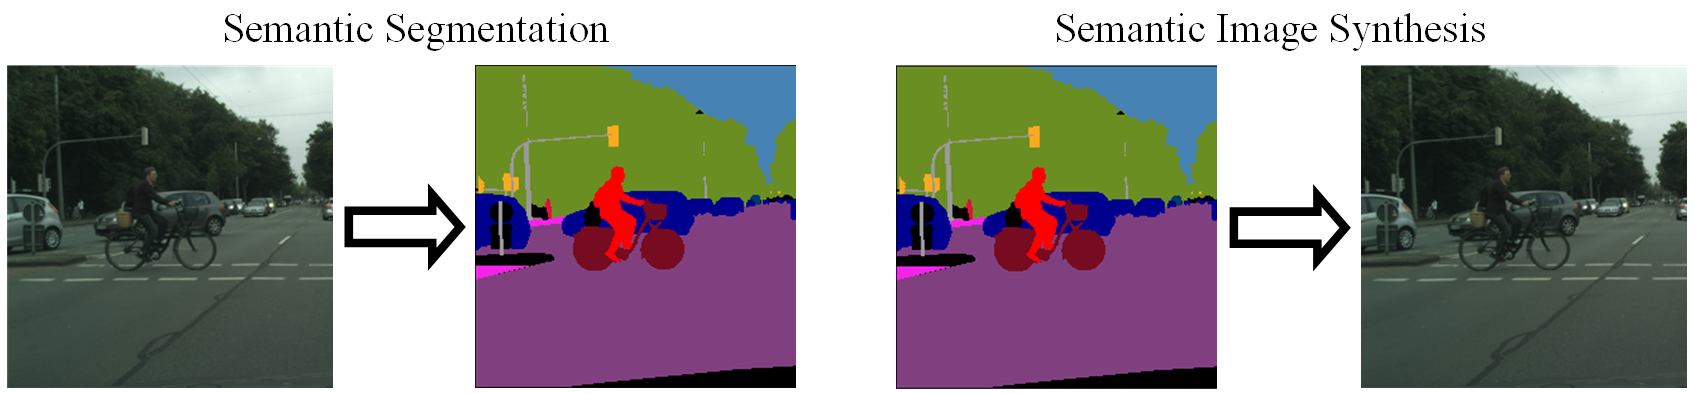
\includegraphics[width=1\textwidth]{Chapters/figures/sem_seg_vs_sem_synth.PNG}
    \caption[Operating principle of semantic segmentation and semantic image synthesis]{Operating principle of semantic segmentation and semantic image synthesis. Images from Cityscapes dataset \cite{cityscapes}}
\end{figure}
%
Two large fields in image-based machine learning are semantic segmentation and semantic image synthesis. In semantic segmentation so-called semantic segmentation networks have the task of a pixel-wise classification of images. In semantic image synthesis – unlike unconditioned image generation \cite{score_3} – images are generated based on a given semantic label map.

In this thesis we show that Score-Based Generative Models, with the help of semantic segmentation networks, are capable of synthesizing realistic looking images based on semantic label maps for various resolutions up to $1024\times512$ and datasets such as Cityscapes \cite{cityscapes}, ADE20K \cite{ade20k} and landscape images scraped from Flickr. We show that the synthesized images for some categories can keep up with or even surpass state of the art generative models such as CRN \cite{crn}, pix2pixHD \cite{pix2pixHD}, and SPADE \cite{spade}, although there is still room for further improvement. We therefore show how the current technique could be optimized in future work to yield even better results. 

\thispagestyle{plain}
The implementation for this work is done with PyTorch and the code is publicly available on GitHub at the following links: 
\begin{itemize}
    \item \url{https://github.com/TimK1998/SemanticSynthesisForScoreBasedModels}
    \item \url{https://github.com/TimK1998/SemanticSegmentation}
\end{itemize}
\thispagestyle{plain}

\chapter{Background}
\section{Neural Networks}
\subsection{The Perceptron}
The basis of each artificial neural network is the \textit{perceptron}. A perceptron essentially is an algorithm that is inspired by biological neurons. The perceptron can therefore be understood as an artificial neuron.

Mathematically, a perceptron processes an input vector $\vec{x}\in\mathbb{R}^n$ and produces an output vector $\vec{y}\in\mathbb{R}^m$. 
%
\begin{figure} \label{fig:2.1}
    \centering
    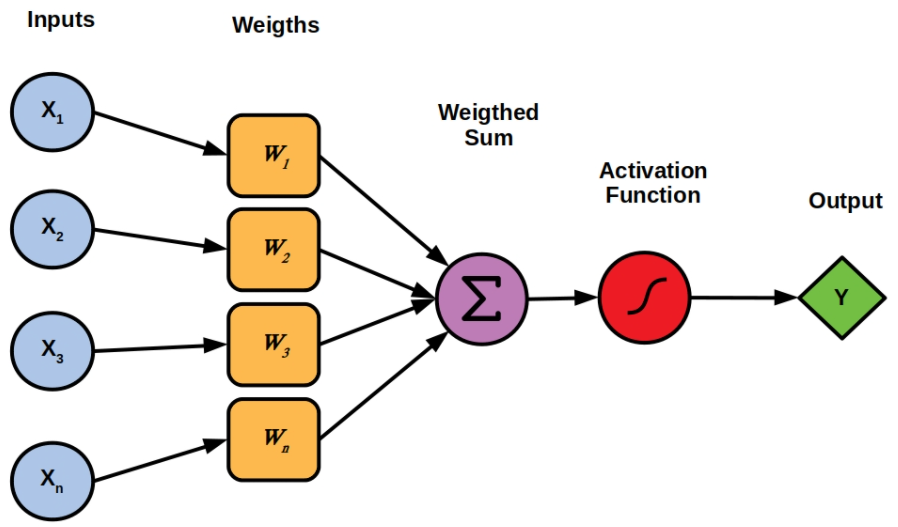
\includegraphics[width=.5\textwidth]{Chapters/figures/perceptron.PNG}
    \caption[Schematic layout of a perceptron]{Schematic layout of a perceptron. Figure from\\ https://starship-knowledge.com/neural-networks-perceptrons.}
\end{figure}
%
In the simplified representation of a perceptron in \hyperref[fig:2.1]{Fig.\,2.1} the inputs $x_i$ $ (i=0,\dots,n)$ are multiplied by weights $w_i$ and then summed. Thereafter a non-linear function is applied to produce the output $y\in\mathbb{R}$. It is the adaption of these weights to a specific problem that is the core of learning in a neural network. A generalization of the transformation described above is given by
%
\begin{equation} \label{equ:2.1}
    \vec{A}\cdot\vec{x}+\vec{b}=\vec{\hat{\vec{y}}}
\end{equation}
%
where $A\in\mathbb{R}^{m\times n}$ is a matrix of weights and $b\in\mathbb{R}^m$ is a bias. Then a non-linear transformation of the form
%
\begin{equation} \label{equ:2.2}
    \vec{y}=\varphi(\hat{\vec{y}})
\end{equation}
%
is applied to the intermediate result $\hat{\vec{y}}$. The non-linear function $\varphi(\cdot)$ is called the \textit{activation function}. This function has the task of mapping the arbitrary output $\hat{\vec{y}}$ from the range $(-\infty,\infty)$ to a more appropriate range. The choice of the activation function depends heavily on the specific architecture of a neural network. Typical choices of activation functions are the Sigmoid, Tanh, Softmax and ReLU functions. As activation functions do not play a big role in this thesis the concrete definition of these functions is left as an exploration to the reader.
%
\subsection{Multilayer Perceptrons} \label{sec:2.1.2}
A \textit{Multilayer Perceptron} is an arrangement of perceptrons in different consecutively interconnected layers. This is what we call a (very basic) \textit{Neural Network}. As depicted in \hyperref[fig:2.2]{Fig.\,2.2} a Multilayer Perceptron is composed of an input layer, one or more hidden layers and an output layer. 
%
\begin{figure} \label{fig:2.2}
    \centering
    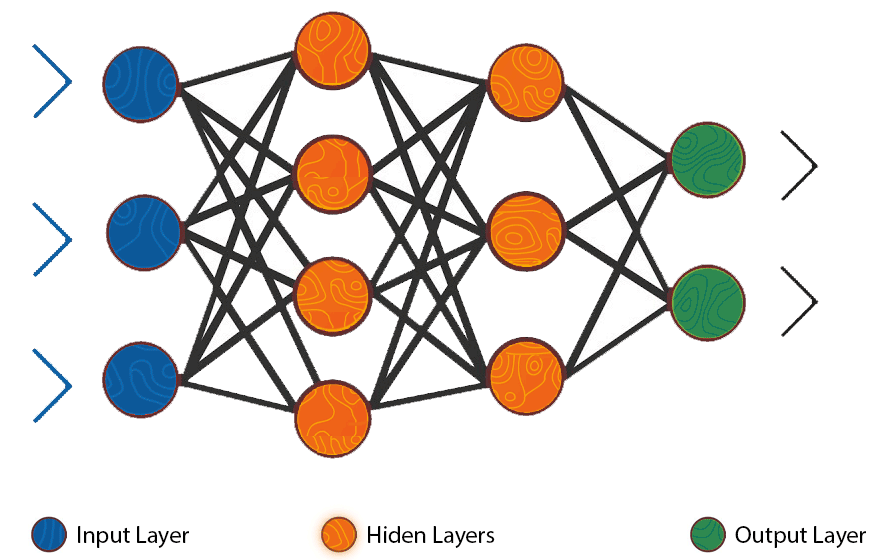
\includegraphics[width=.5\textwidth]{Chapters/figures/multilayer_perceptron.PNG}
    \caption[The Multilayer Perceptron]{The Multilayer Perceptron. Figure from\\ https://cdn.analyticsvidhya.com/wp-content/uploads/2020/02/ANN-Graph.gif}
\end{figure}
%
The output of a layer is connected to the input of the next layer (here: fully connected). The hidden layers can perform various tasks and some of them are presented in \hyperref[sec:2.1.3]{Sec.\,2.1.3}.

During training the learning process of such a neural network consists of three parts which are computed iteratively: the \textit{forward pass}, the \textit{loss calculation} and the \textit{backward pass}. In the forward pass, the input values get processed by the different layers of the neural networks to then produce an output. The loss calculation then computes how good this output is in relation to some optimal output for the given input. This is the concept of \textit{supervised learning}. There is a variety of so-called \textit{loss functions} for the calculation of losses, some of them will be discussed later in this thesis. The computed loss is then back-propagated through the network to update the parameters of each perceptron in each layer. This is the process of artificial learning. Back-propagation often works in the sense of a gradient descent. Since the loss is to be minimized, the influence of all individual parameters on the loss is then derived and adjusted according to the resulting gradient. 

Usually a batch of data is processed simultaneously by the network. While processing the whole dataset at once would lead to faster converging and overall better results in optimization with gradient decent, a larger batch size comes with a much higher vRAM cost during training. Therefore one often decides to use a mini-batch of data which makes the best possible use of the memory of the graphics card. The process of forward pass, loss computation and backward pass of one batch is then called an \textit{iteration} or a \textit{step}. After each batch has been processed in a dataset, an \textit{epoch} has passed.
%
\subsection{Common Layers in Neural Networks} \label{sec:2.1.3}
Depending on the task of the neural network, different layers of perceptrons are used. The most common ones are \textit{Fully Connected Layers}, \textit{Normalization Layers}, \textit{Convolutional Layers}, \textit{Pooling 
Layers} and \textit{Dropout \cancel{Layers}}. It is important to note that the choice of layers for a specific problem is \textbf{not} trivial! In fact, often it is not even clear why a specific layer is good for a specific task. Furthermore, when training a neural network, it is – in general – impossible to have any insight on how the neural network learned the task.
%
\subsubsection{Fully Connected Layers}
A fully connected layer is the easiest layer for neural networks. In this layer, the output of every perceptron in one layer is connected to the input of every perceptron in the next layer. Mathematically, this describes a linear operation between the perceptrons of two layers. Although fully connected layers are in theory able to fit every problem quite well (see Universal Approximation Theorem, e.g. \cite{universal_appr_theorem}) ,they cannot be used excessively. Considering a $128\times128$ pixel RGB image leads to $4,831,838,208$ parameters to learn for two fully connected layers. Learning such a high number of parameters (weights) is computationally very expensive and often not feasible.
%
\subsubsection{Normalization Layers}
Normalization layers normalize the given inputs. There are several normalization techniques that depend on the choice of what to normalize. Take Batch Normalization (BN) \cite{batch_norm} as an example. Suppose the image data is of the form $(N, C, W, H)$ where $N$ is the batch size, $C$ is the channel number (e.g. $3$ for RGB images) and $W$ and $H$ are width and height respectively. Then BN normalizes $(N, W, H)$ for each $C$ by transforming the input $\vec{x}$ in the following way:
%
\begin{equation} \label{equ:2.3}
    \mu_B=\frac{1}{N}\sum_{i=1}^Nx_i, \quad\sigma_B^2=\frac{1}{N}\sum_{i=1}^N(x_i-\mu_B)^2\quad \Longrightarrow\quad y_i=\gamma\frac{x_i-\mu_B}{\sigma_B}+\beta,
\end{equation}
%
where $\gamma$ and $\beta$ are learnable parameters of the layer. Depending on the dimensions of the input that get normalized there is also \textit{Channel Norm}, \textit{Instance Norm} and \textit{Group Norm}. Normalization layers are used to improve the stability, speed and performance of neural networks.
%
\subsubsection{Convolutional Layers}
The Convolution Layer might be the most important layer in computer vision and gives rise to the category of \textit{Convolutional Neural Networks} (CNNs) \cite{cnn}. This type of neural networks makes extensive use of convolutional layers and is an important concept in computer vision tasks as it is very good at capturing image details \cite{deep_image_prior}.

A Convolutional Layer is especially useful to extract features from images. For example, these features could be lines in different direction but as mentioned above, normally we do not know what information (features) a neural network learns in a (convolutional) layer. In general, one can only say that in a CNN of subsequent Convolutional Layers the upper layers learn more simple features such as lines and the deeper layers learn more complex features, e.g. how a car looks like. This characteristic is called \textit{receptive field} and is due to the fact that a pixel of the first convolutional layer contains information only from, for example, $9$ pixels of the image for a $3\times3$ convolution, while a deeper convolutional layer contains information from many more pixels of the image.

As the Convolutional Layer is most often used for image feature extraction, the \textit{2D-Convolution Layer} is the most popular Convolution Layer and is defined by a 2-dimensional convolution
%
\begin{equation}
    y_{i,j}=(\vec{x}\ast\vec{f})_{i,j}=\sum_{c=1}^{C}\sum_{h=1}^{H_f}\sum_{w=1}^{W_f}\vec{f}_{c,h,w}\vec{x}_{i+h-1,j+w-1,c}
\end{equation}
%
for an input of size $(C,H,W)$. Essentially this operation can be understood as applying a filter $\vec{f}$ of size $(C, H_f, W_f)$ to each part of the image. For each position of the filter the corresponding values in the image are multiplied with the learned weights in the filter and then summed up. These summed values for each filter position then form a new output. An illustration of this process is shown in \hyperref[fig:2.3]{Fig.\,2.3}.
%
\begin{figure} \label{fig:2.3}
    \centering
    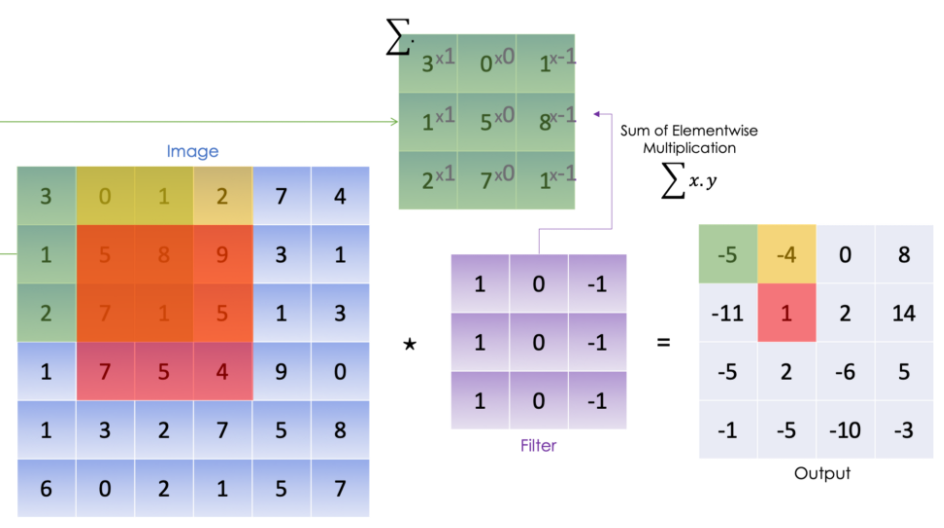
\includegraphics[width=.65\textwidth]{Chapters/figures/convolution.PNG}
    \caption[Operation principle of Convolutional Layers]{Operation principle of Convolutional Layers. Figure from\\ https://towardsdatascience.com/convolutional-neural-networks-mathematics-1beb3e6447c0.}
\end{figure}
%
\subsubsection{Pooling Layers}
As we have seen, Convolutional Layers summarize and learn specific features in an input image. These feature maps are very sensitive to the location of the features in the input. To make the feature maps more robust to changes in the position of the feature in the image, Pooling Layers are deployed. A Pooling Layer works by dividing the feature map into slices of size $n\times m$. These slices are then condensed to a single scalar value by a pooling operation. Popular pooling operations are \textit{max pooling} and \textit{average pooling}, which given a slice $\tilde{\vec{x}}=(x_{ij})$ for $i=1,\dots,n$ and $j=1,\dots,m$ compute the following:
%
\begin{align}
    \text{max pooling:}\quad&f(\tilde{\vec{x}})=\underset{i,j}{\max}(x_{ij})\\
    \text{average pooling:}\quad&f(\tilde{\vec{x}})=\frac{1}{n\cdot m}\sum_{i=1}^n\sum_{j=1}^mx_{ij}
\end{align}

It should be noted that pooling layers are often also used as downsampling layers.
%
\subsubsection{Dropout \cancel{Layers}}
Dropout can be applied to any other layer type and has no learnable parameters. Dropout therefore is no real layer. During training, specified by a dropout probability $p$, parameters are randomly set to $0$. The purpose of dropout is to prevent model overfitting, i.e. preventing the model from memorizing instead of learning a dataset.
%
\subsection{Model Objectives}
The concept of \textit{model} is very important in Deep Learning. A model can be understood as a superordinate concept to a concrete network implementation. We denote a model as $s_\theta(\vec{x})$, where $\vec{x}$ is the data input and $\theta$ is the set of all learnable parameters.

To define the task of an model, an \textit{objective} is set up. An objective is a function that represents the task the model is trying to accomplish. Usually, the task is represented such that the objective function is to be minimized or maximized. As an example, imagine a model that has the task to approximate (learn) the function $f(x)=x^2$. The objective of this task can be chosen as
%
\begin{equation} 
    \theta^*=\underset{\theta}{\arg \min}\norm{x^2-s_\theta(x)}.
\end{equation}
%
The notation is interpreted in the following way: The optimal parameters $\theta^*$ are the ones that minimize the distance between $x^2$ and the model $s_\theta(x)$. This gives rise to the definition of the optimal model $s_{\theta^*}(\vec{x})$ which by definition solves the task perfectly. When describing the learning process of a model it is then stated that the trained model fulfills $s_\theta(\vec{x})\approx s_{\theta^*}(\vec{x})$ or in the case of our example $s_\theta(x)\approx s_{\theta^*}(x)\overset{!}{=}x^2\,\forall x\in\mathbb{R}$.

If the model is dependent on additional information, e.g. time $t$, the model is expanded to $s_\theta(\vec{x}; t)$. 
%
\section[Data Distributions and Probability Density Functions]{Data Distributions and Probability Density Functions%
    \sectionmark{Data Distributions and PDFs}} \label{sec:3.3}
\sectionmark{Data Distributions and PDFs}
Statistical Data Distributions and Stochastic Processes play a large role in the theory behind Score-Based Generative Models. When describing the goal of a model it is often said that the model tries to learn the data distribution of a dataset. The data distribution $p_{data}(\vec{x})$ of a dataset $D\subset\mathbb{R}^d$  describes how the data $\vec{x}\in D$ is distributed in relation to certain descriptive variables. The data distribution describes \textit{all} possible data, e.g. all images of cars. Obviously, a real dataset cannot contain an infinite number of images. That is why the data distribution often is impossible to know. The real dataset has the following relation to the data distribution: $D=\{\vec{x}_i\}_{i=1}^N\overset{i.i.d}{\sim}p_{data}(\vec{x})$. The $\sim$ means that $D$ is distributed as $p_{data}$ and $N$ denotes the finite number of data in the dataset. $D\subset D^*$ where $D^*$ is the infinite, perfect dataset. In order for the model being able to learn the data distribution from a subset of $D^*$, the data in $D$ must be \textit{independently and identically distributed} (i.i.d) which essentially means that $D$ should replicate the data distribution as good as possible.

Each distribution can also be represented as a \textit{probability density function} (pdf) $p(\vec{x})$. While a data distribution shows the frequency of certain variables and often is discrete a pdf is a continuous function describing the probability of the variables in a distribution. 




\chapter{Related Work}

\section{Semantic Segmentation} \label{sec:3.1}
A large field of models in Deep Learning are discriminative models. A simple version of a discriminative model would be a classifier. A classifier given an input $\vec{x}$ outputs a scalar class value $y\in\vec{y}$ of the input where $\vec{y}$ is a set of classes (which are also called labels). The simplest classifier would be a binary classifier that places an input into one of two classes, e.g. deciding if an image shows a cat or a dog. More advanced classifiers identify way more classes. A classical example would be a classifier trained on the CIFAR-10 dataset \cite{cifar10}, which contains millions of $32\times32$ pixel images categorized by 10 classes (car, airplane, dog, $\dots$).

The above described classifiers always assign one scalar value to an input. Semantic Segmentation Networks also assign scalar values, but not one value per image, but one value per pixel! This already reveals a lot about the application of such networks. They operate on images and their task is to assign each pixel in the image a class. For example, given the image of a street scene a semantic segmentation network tries to classify each individual pixel as part of a car, a street, a building, $\dots$\,.

There are also modifications of semantic segmentation for example instance segmentation. In instance segmentation, not only is each pixel assigned a class, but also the different instances of objects in an image are specified. An overview of semantic segmentation and related techniques is shown in \hyperref[fig:3.1]{Fig.\,3.1}
%
\begin{figure} \label{fig:3.2}
    \centering
    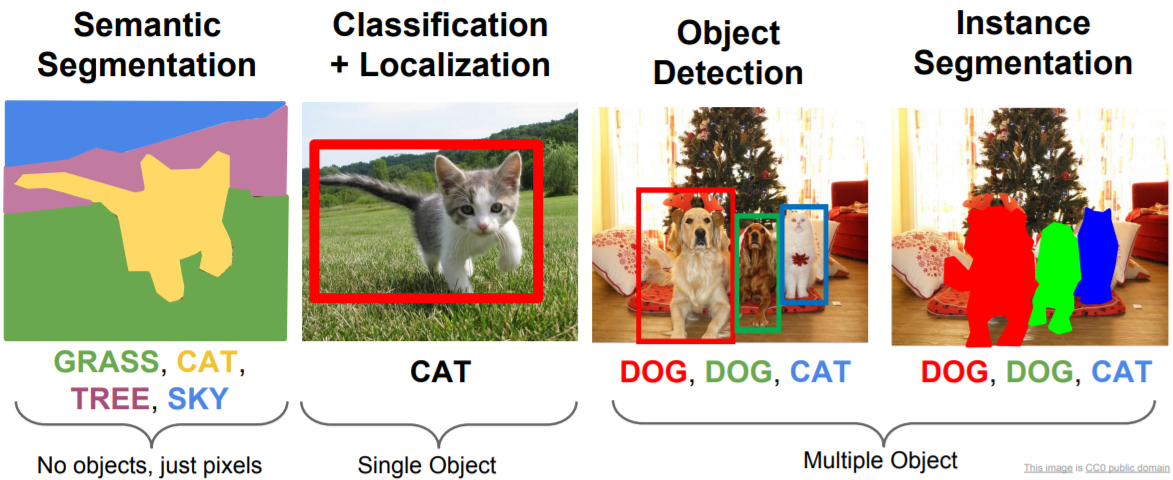
\includegraphics[width=.8\textwidth]{Chapters/figures/sem_seg.PNG}
    \caption{Overview of various computer vision tasks}
\end{figure}
%

As we will see in \hyperref[sec:4.5]{Sec.\,4.5} and \hyperref[chap:5]{Chapter 5}, semantic segmentation networks are necessary to make semantic image synthesis possible with Score-Based Generative Models. Therefore, those models used in later work are briefly explained below:

\subsection{FCN}
\subsection{U-Net} %1-2

%%%%%%%%%%%%%%%%%%%%%%%%%%%%%%%%%%%%%%%%%%%%%%%%%%%%%%%%%%%%%%%%%%%%%%%%%%%%%%%%%%%%%%%%%%%%
\section[Generative Modeling – VAEs and GANs]{Generative Modeling – VAEs and GANs%
    \sectionmark{Generative Modeling}}
\sectionmark{Generative Modeling}
There are mainly two types of models: \textit{Generative Models} and \textit{Discriminative Models}. The latter discriminate between different kind of data instances, e.g. discriminate images of cats and dogs. Semantic Segmentation Models (\hyperref[sec:3.1]{Sec.\,3.1}) are discriminative models. Given a data instance $\vec{x}$ and a set of labels $\vec{y}$ conditional models learn the conditional probability $p(\vec{y}|\vec{x})$. Generative model generate new data instances. They capture the joint probability $p(\vec{x},\vec{y})$ or $p(\vec{x})$ if there are no labels. In general generative models are a lot harder than discriminate models. There are various approaches to generative modeling, the most popular being Variational Autoencoders (VAEs) and Generative Adversarial Networks (GANs).

\subsubsection{Variational Autoencoders}
Although VAEs \cite{vae_original} do not play a major role in this thesis, they are briefly discussed due to their strong influence in modern generative modeling. In order to understand VAEs one must first understand what an autoencoder is. Autoencoders tackle the problem of encoding and decoding data with minimum information loss. Data generally is classified by some abstract features which often form a high dimensional space. The task of an autoencoder is to learn to reduce the dimensionality of this high dimensional features by selecting important old features (selection) or creating less, new features based on the old features (extraction). The arising feature space is called \textit{latent space} which essentially only contains the most important features of the input data. To learn such an encoding the autoencoder network consists of an encoder network $E(\vec{x})$ and a decoder network $D(\vec{x})$. An input $\vec{x}$ is first encoded by the encoder to a low dimensional value $\vec{z}$ which then is decoded by the decoder to an output $\tilde{\vec{x}}$ of the same dimension as the input. Thereafter the input $\vec{x}$ is compared to the output $\tilde{\vec{x}}$ and the network gets punished for differences between input and output.

An autoencoder thus learns to compress and decompress data in the best possible way without loss of information. A na\"{i}ve way to now generate new data via a trained autoencoder is to use the decoder to decode a random sample from the latent space. The problem with this approach is that the autoencoder learns to best possible compress the data. As a consequence we cannot sample from the latent space because the distribution in latent space has no meaning w.r.t the real data. For example, if you decode the image of a car into the latent space and then change the latent representation of the car just a little, after decoding you will most likely see noise instead of an image of a new car. In mathematical terms the latent space of an autoencoder is not regularized.

A VAE solves this problem by ensuring that the latent space has good properties that enable generative modeling while still learning to encode the data in an efficient way. In order to do so the encoder of a VAE does not encode an input $\vec{x}$ to a single value but to a distribution in latent space $p(\vec{z}|\vec{x})$. The decoder then decodes a sample $\vec{z}\sim p(\vec{z}|\vec{x})$ to an output $\tilde{\vec{x}}$ which is compared to the output to compute a reconstruction loss. Furthermore a regularization loss is computed assuring that $p(\vec{z}|\vec{x})\sim\mathcal{N}(\vec{0},\vec{I})$. The regularized latent space has the very useful property that similar data is close together. So now if the decoder is given a slightly different latent representation of a car, it would decode it into a new image of a car. An overview of the VAE network architecture can be seen in \hyperref[fig:3.1]{Fig.\,3.1}
%
\begin{figure} \label{fig:3.2}
    \centering
    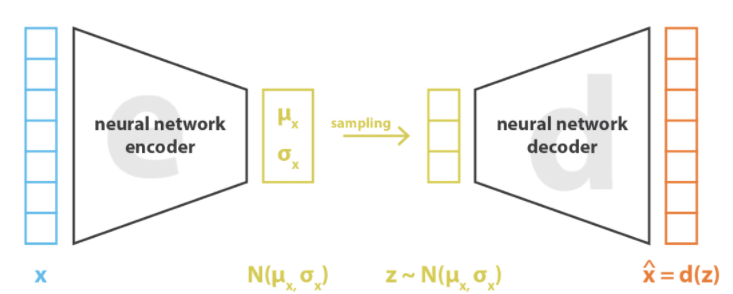
\includegraphics[width=.65\textwidth]{Chapters/figures/vae.PNG}
    \caption{Basic VAE model architecture}
\end{figure}
%
\subsubsection{Generative Adversarial Networks}
GANs were proposed in 2014 \cite{gan_original} and have since seen great success and a lot of adaptions. GANs work by combining two models: A generator model and a discriminator model. These two models are trained at the same time and have an adversarial relationship. Adversarial in that sense means that the generator and discriminator have opposing objectives. 

The generator $G(\vec{x})$ has the task of generating samples of the data distribution $p_{data}(\vec{x})$. The discriminator $D(\vec{x})$ has the role of distinguishing the generated data $\tilde{\vec{x}}$ from the real data $\vec{x}$. So to say the task of the generator is to best possible trick the discriminator that at the same time has the task to best possible decide if an image is real or fake (generated). If the discriminator correctly identifies a generated image as fake the generator is punished to produce better images. Obviously, "better" just means that the images are more likely to fool the discriminator, which does not necessarily equate to a real-looking image. When the discriminator is deceived by the generator, it is punished to better discriminate real and fake images. While the GANs can produce excellent samples and are fast at sampling, it's easy to imagine how hard it is to train two networks at the same time. If not properly adjusted training quickly becomes unstable.

The absolute error of the discriminator can be written in the following way:
%
\begin{equation}
    E(G,D)=\frac{1}{2}\left(\mathbb{E}_{\vec{x}\sim p_{t}}[1-D(\vec{x})]+\mathbb{E}_{\vec{x}\sim p_{z}}[D(G(\vec{z}))]\right)
\end{equation}
%
Here $\vec{x}$ is a input to the discriminator and $\vec{z}$ is a random input to the generator. Rewriting $G(\vec{z})$ as an input to the discriminator yields
%
\begin{equation} \label{equ:3.2}
    E(G,D)=\frac{1}{2}\left(\mathbb{E}_{\vec{x}\sim p_{t}}[1-D(\vec{x})]+\mathbb{E}_{\vec{x}\sim p_{g}}[D(\vec{x})]\right),
\end{equation}
%
where $\vec{x}$ can either be a real input ($\vec{x}\sim p_t$) or a generated input ($\vec{x}\sim p_g$). Therefore in \hyperref[equ:3.2]{Equ.\,3.2} the left term describes the error of falsely classifying a real image as generated and the right term describes the error of falsely classifying a generated image as real. From this it can be deduced that the perfect discriminator $D^*(\vec{x})$ classifies a real image as $1$ and a fake image as $0$. 

The total model objective of GANs can be written as 
%
\begin{equation}
    \underset{G}{\max}\left(\underset{D}{\min}\,E(G,D)\right),
\end{equation}
%
which can be interpreted as the discriminator trying to minimize its error, while at the same time the generation tries to maximize the discriminator's error. A sketch of the training procedure is shown in \hyperref[fig:3.2]{Fig.\,3.2}. 
%
\begin{figure} \label{fig:3.2}
    \centering
    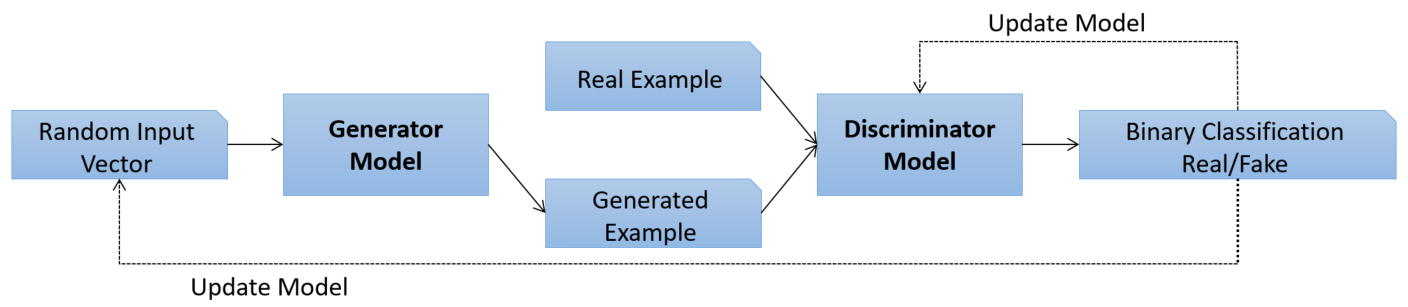
\includegraphics[width=.9\textwidth]{Chapters/figures/gan.PNG}
    \caption{Basic GAN model architecture}
\end{figure}
%

In this thesis the results of our score-based generative semantic image synthesis model are compared with the results of state-of-the-art GANs. All GAN models used for comparison are briefly explained below:

\subsection{Cascaded Refinement Networks}
\subsection{pix2pixHD} 
\subsection{SPADE} 


\chapter{Score-Based Generative Models} %5-7
\chaptermark{SGM}
As we have seen in the preceding chapters there is quite a large range of models designed to generate data such as images, audio, or video. Despite this high diversity, only some of them – in particular GANs and VAEs – achieved outstanding success \cite{biggan, vqvae2}, on the basis of which they were heavily improved in the last years. It is therefore quite difficult to come up with a new model that is able to quickly keep up with these highly adapted models. The fact that in this harsh environment \textit{Score-Based Generative Models} \cite{score_1, score_3, score_2} were able to achieve state-of-the-art results explains why they recently gained a lot of attention and makes them a new promising contender to the field of well-established generative models.

As Score-Based Generative Models were going through a lot of changes since the first publication, the next sections chronologically explain Score-Based Generative Models and their evolution in detail. In \hyperref[sec:4.1]{Sec.\,4.1} a brief overview of the core concepts of Score-Based Generative Models is given, followed by \hyperref[sec:4.2]{Sec.\,4.2} explaining why this core concept fails when being used without adaptions. \hyperref[sec:4.3]{Sec.\,4.3} then presents how adding noise of discrete noise scales to the data distribution makes Score-Based Generative Modeling feasible, after which \hyperref[sec:4.4]{Sec.\,4.4} generalizes this concept by introducing continuous noise governed by a Stochastical Differential Equation (SDE). Finally, in \hyperref[sec:4.5]{Sec.\,4.5} the theory behind controllable generation is presented.

%%%%%%%%%%%%%%%%%%%%%%%%%%%%%%%%%%%%%%%%%%%%%%%%%%%%%%%%%%%%%%%%%%%%%%%%%%%%%%%%%%%%%%%%%%%%%%%%
\section{The idea behind Score-Based Generative Models} \label{sec:4.1}
\sectionmark{The idea behind SGM}
In general, the most basic Score-Based Generative Model consists of two core ideas: First, estimating the score $\nabla_{\vec{x}}\log p(\vec{x})$ of an unknown data distribution $p_{data}(\vec{x})$ of a dataset $\{\vec{x}_i\in \mathbb{R}^d\}_{i=1}^N$ of $N$ i.i.d samples. This process is referred to as \textit{Score Matching} \cite{score_matching_original}. And second, using \textit{Langevin Dynamics} \cite{langevin1, langevin2} to sample from the data distribution by starting with an initial value $\tilde{\vec{x}_0}$ from a prior distribution $\pi(\vec{x})$. This value is then gradually transformed by $T$ recursive steps of Langevin Dynamics and will finally come out as $\tilde{\vec{x}}_T$ where $p(\tilde{\vec{x}}_T)\approx p_{data}(\vec{x})$, which makes it a nearly perfect sample of $p_{data}(\vec{x})$. The resulting generative modeling framework is called \textit{Score Matching Langevin Dynamics} (SMLD).
%
\subsection{Score Matching} \label{sec:4.1.1}
This section gives an overview of Score Matching and how this technique can be used to get an objective for a score estimator, i.e. the model that is trained to estimate the score $\nabla_{\vec{x}}\log p_{data}(\vec{x})$ of the data distribution $p_{data}(\vec{x})$. The section is mathematically fairly intensive, and for that reason the main goal of this section is to provide a good feeling for why using the estimation of the score function as a model objective is a reasonable idea.

Score Matching \cite{score_matching_original} is a technique that originates from probabilistic models and their difficulties to be trained on an unnormalized probability density function $\tilde{p}(\vec{x})$ of a data distribution $p_{data}(\vec{x})$. The task of such a model $p_\theta(\vec{x})$ is to learn parameters $\theta$ such that $p_\theta(\vec{x})=p_{data}(\vec{x})$ where $p_{data}(\vec{x})$ is the normalized density function defined as
%
\begin{equation}
    p_{data}(\vec{x})=\frac{\tilde{p}(\vec{x})}{Z},\quad Z=\int\tilde{p}(\vec{x})d\vec{x}\,.
\end{equation}
%
$Z$ is called the partition function and can be understood as a normalization constant. It is this partition function $Z$ that causes the models difficulty to achieve its task. This is because the computation of $Z$ is intractable, meaning that it cannot be solved in polynomial time or rather its complexity is at least $\mathcal{O}(k^n)$, where $k>1$ is some constant and $n\in\mathbb{N}$ is the length of an input. The reason to use the score function to overcome this problem can be easily seen by using the calculation rules for logarithms to get $\log p(\vec{x})=\log\tilde{p}(\vec{x})-\log Z$. It is therefore obvious that the score function $\nabla_{\vec{x}}\log p(\vec{x})$ does not depend on the intractable partition function $Z$.

Score Matching uses this fact by minimizing the Fisher divergence between $p_{data}(\vec{x})$ and $p_\theta(\vec{x})$, which is defined as
%
\begin{equation} \label{equ:4.2}
    L(\theta)\triangleq\frac{1}{2}\mathbb{E}_{p_{data}}[\norm{s_\theta(\vec{x})-\nabla_{\vec{x}}\log p_{data}(\vec{x})}^2_2],
\end{equation}
%
where $s_\theta(\vec{x})\triangleq\nabla_{\vec{x}}\log p_\theta(\vec{x})$ and $\norm{\cdot}_2$ is the Euclidean norm. From here on, we now begin to transition from the probabilistic model $p_\theta(\vec{x})$ to the score model $s_\theta(\vec{x})$. \hyperref[equ:4.2]{Equ.\,4.2} is the formulation of Score Matching which can be used in an integrated form as part of the model objective for probabilistic models. But beyond that Score Matching can also be used as a standalone model objective for the so-called \textit{Score-Based Models}.

Ultimately, both probabilistic models and score-based models learn the data distribution so that it is possible to generate samples from it. However probabilistic models aim to learn the data distribution itself. Score-based models ($s_\theta(\vec{x})$) aim to learn the score of the data distribution. In order to train a score-based model, we have to reformulate the objective in \hyperref[equ:4.2]{Equ.\,4.2} as it is still not readily usable for leaning score-models because the data distribution $p_{data}(\vec{x})$ is typically unknown and so is $\nabla_{\vec{x}}\log p_{data}(\vec{x})$. 

To address the problem of the unknown data distribution, \textit{Denoising Score Matching} \cite{denoise_score} was proposed. Denoising Score Matching introduces noise to \hyperref[equ:4.2]{Equ.\,4.2} so that $\nabla_{\vec{x}}$ does not operate directly on the unknown distribution. A noise distribution $q_\sigma(\tilde{\vec{x}}|\vec{x})$ is applied to the data distribution to get a perturbed data distribution $q_\sigma(\vec{x})=\int q_\sigma(\tilde{\vec{x}}|\vec{x})p_{data}(\vec{x})d\vec{x}$. When the noise is small ($q_\sigma(\vec{x})\approx p_{data}(\vec{x})$) then $s_\theta(\vec{x})=\nabla_{\vec{x}}\log q_\sigma(\vec{x})\approx\nabla_{\vec{x}}\log p_{data}(\vec{x})$ holds true. The objective of Denoising Score Matching follows as
%
\begin{equation} \label{equ:4.3}
    \theta^*=\underset{\theta}{\arg\min}\frac{1}{2}\mathbb{E}_{q_\sigma(\tilde{\vec{x}}|\vec{x})p_{data}(\vec{x})}[\norm{s_\theta(\vec{x})-\nabla_{\vec{x}}\log q_\sigma(\tilde{\vec{x}}|\vec{x})}^2_2].
\end{equation}
%
In conclusion, \hyperref[equ:4.3]{Equ.\,4.3} is the training objective for score-based models that is further used throughout this thesis. Nevertheless, there are also other Score Matching techniques such as \textit{Sliced Score Matching} \cite{song2019sliced} that could be used, but it turns out that Denoising Score Matching is considerably faster. The objective of Score-Based Models (\hyperref[equ:4.2]{Equ.\,4.2}) has several desirable properties which makes it a reasonable approach for a generative model. As shown above the objective does not rely on the intractable partition function $Z$. Therefore, the objective is almost always tractable which has the implications that there is no special model architecture necessary. Furthermore, the objective can be optimized without adversarial training (\hyperref[sec:gans]{Sec.\,3.2}) making it easier and more stable to train.

\subsection{Langevin Dynamics} \label{sec:4.1.2}
As described in \hyperref[sec:4.1.1]{Sec.\,4.1.1} a score-model is tasked to estimate the score of the unknown data distribution $p_{data}(\vec{x})$ of a dataset. However, the score of a distribution is not yet a generated image. Instead, as it is the \textit{gradient} of the (log) data distribution it can be utilized to sample from $p_{data}(\vec{x})$ by transforming a value $\tilde{\vec{x}}_0$ of a prior distribution $\pi(\vec{x})$ to be part of the data distribution, following the gradient (the score) of the data distribution. There are some restrictions to what the prior distribution should look like but for the considerations of score-based models the prior distribution is just Gaussian noise, so $\pi(\vec{x})\sim\mathcal{N}(\vec{x}, \vec{0}, \vec{I})$.

The process used for sampling is based on \textit{Langevin Dynamics}, a concept from physics, that was adopted to machine learning \cite{langevin1, langevin2}. In Physics, the \textit{Langevin Equation} describes particles moving in a potential which additionally are subject to random forces. This process is called \textit{Brownian Motion}. The Langevin equation reads as 
%
\begin{equation} \label{equ:4.4}
    \lambda \frac{\vec{x}(t)}{dt}=-\nabla_{\vec{x}} V(\vec{x}(t))+\vec{\eta}(t),
\end{equation}
%
where $V$ is the potential the particle is moving in, $\vec{x}(t)$ is the particle's position and $\vec{\eta}(t)$ is white noise. Commonly \hyperref[equ:4.4]{Equ.\,4.4} is written as an (Itô)-Stochastical Differential Equation (SDE)
%
\begin{equation} \label{equ:4.5}
    d\vec{x}(t)=\underbrace{-\nabla_{\vec{x}} V(\vec{x}(t))\,dt}_\text{drift term}+\underbrace{\sqrt{2}\,d\vec{w}}_\text{diffusion term},
\end{equation}
%
with a drift term and a diffusion term. $\vec{w}$ denotes the \textit{Wiener Process} \cite{gardiner} which can be interpreted as the derivative of white noise. It is important to note that the positions of particles described by \hyperref[equ:4.5]{Equ.\,4.5} are distributed according to some probability density function $p(\vec{x})$ for all times $t\geq0$. This has some very useful consequences: We can choose the potential $V$ in such a way that the underlying probability density function is $p_{data}$. In this case we can sample from $p_{data}$.

To achieve the state where the particles position described by the Langevin Equation are distributed by $p_{data}$ we have to choose $V(\vec{x})=-\log p_{data}({\vec{x}})$. Inserting $V(\vec{x})$ into \hyperref[equ:4.5]{Equ.\,4.5} results in
%
\begin{equation} \label{equ:4.6}
    d\vec{x}(t)=\nabla_{\vec{x}}\log p_{data}(\vec{x})dt+\sqrt{2}\,d\vec{w}.
\end{equation}
%
Now, the connection between Sampling with Langevin Dynamics and Score Matching (\hyperref[sec:4.1.1]{Sec.\,4.1.1}) can be seen. If the score of the data distribution is known we can sample from this distribution by using \hyperref[equ:4.6]{Equ.\,4.6}. For now, $\vec{x}(t)$ was the position of a physical particle but \hyperref[equ:4.6]{Equ.\,4.6} is applicable for any $d$-dimensional data $\vec{x}(t)\in\mathbb{R}^d$, e.g. images. To use \hyperref[equ:4.6]{Equ.\,4.6} in the context of machine learning we cannot directly use the SDE as it describes continuous steps of infinitesimal size. We therefore discretize the SDE to discrete steps which can then be calculated by a computer. The resulting discretization in \hyperref[equ:4.7]{Equ.\,4.7} is called the Euler-Maruyama discretization of the SDE.
%
\begin{equation} \label{equ:4.7}
    \tilde{\vec{x}}_t=\tilde{\vec{x}}_{t-1}+\frac{\epsilon}{2}\nabla_{\vec{x}}\log p_{data}(\tilde{\vec{x}}_{t-1})+\sqrt{\epsilon}\,\vec{z}_t
\end{equation}
%
\hyperref[equ:4.7]{Equ.\,4.7} is a recursive algorithm that can be used to sample from $p_{data}$. Here $\tilde{\vec{x}}_0$ is a value from the prior distribution given above and the "$\sim$" above the $\vec{x}$ shows that $\tilde{\vec{x}}$ is not in the dataset nor described by the data distribution $p_{data}(\vec{x})$ but a random initial sample. Furthermore $z_t\sim\mathcal{N}(0, I)$ is Gaussian noise and $\epsilon$ is the step size of the algorithm. The sample after $T$ steps is a perfect sample of $p_{data}$ when $T\rightarrow\infty$ and $\epsilon\rightarrow0$. For application of this algorithm $T\gg0$ and $\epsilon\ll1$ are assumed.

Recapitulating what the algorithm does, one can look at \hyperref[fig:4.1]{Fig.\,4.1}. The lines in the left image show a particle moving randomly according to \hyperref[equ:4.5]{Equ.\,4.5}. In the background the underlying (heart-shaped) data density function  is represented and in the right image samples are shown, where each of the dots is an initial sample from the prior distribution that was transformed using \hyperref[equ:4.7]{Equ.\,4.7}. When applying \hyperref[equ:4.7]{Equ.\,4.7} to infinite values from the prior distribution this process can be thought of as transforming one distribution to another one. As a side note, the formulation of this integrated process is given by the \textit{Fokker-Planck-Equation} \cite{gardiner} – another important equation in physics. For the purposes of score-based models only a one-by-one application of \hyperref[equ:4.7]{Equ.\,4.7} is needed, essentially transforming one image from a noise distribution to an image that looks like it belongs to the data distribution of the target dataset.
%
\begin{figure}[] \label{fig:4.1}
    \centering
    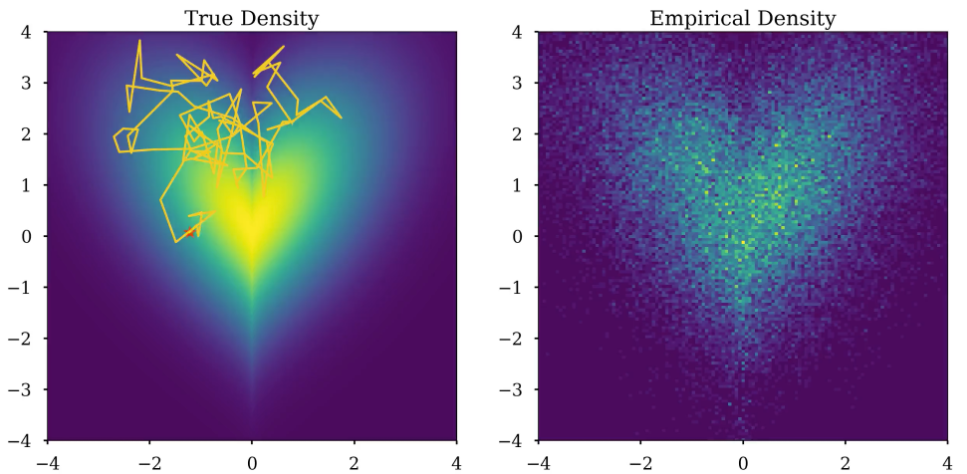
\includegraphics[width=.8\textwidth]{Chapters/figures/langevin.PNG}
    \caption[Application of Langevin Dynamics sampling]{Application of Langevin Dynamics sampling. Figure from\\ https://abdulfatir.com/Langevin-Monte-Carlo/}
\end{figure}
%%%%%%%%%%%%%%%%%%%%%%%%%%%%%%%%%%%%%%%%%%%%%%%%%%%%%%%%%%%%%%%%%%%%%%%%%%%%%%%%%%%%%%%%%%%%%%
\section{Hindrances of a na\"{i}ve application} \label{sec:4.2}
While this general concept looks quite appealing to use as the basis for a generative model, in its na\"{i}ve application it might fail for datasets containing real world data. The authors of \cite{score_1} discuss two hindrances preventing this na\"{i}ve application, which both are bypassable by adding random noise to the data. These bypasses also have some consequences on Score Matching and Langevin Dynamics which will be discussed in \hyperref[sec:4.3]{Sec.\,4.3}. It should be noted, however, that the final score-based model (\hyperref[sec:4.4]{Sec.\,4.4}) which we will derive in the following two sections can also be derived from considerations other than those described in this section.
%
\subsection{The manifold hypothesis} \label{sec:4.2.1}
The problems in both \hyperref[sec:4.2.1]{Sec.\,4.2.1} and \hyperref[sec:4.2.2]{Sec.\,4.2.2} originate from a similar source: The data density of a dataset of real world data. The manifold hypothesis states that real world high-dimensional data lies on low-dimensional manifolds embedded within the high-dimensional space which is called the ambient space. To further explain this hypothesis with an example, one can imagine a dataset of black and white images, each image being $m\times n$ pixels in size. The ambient space – the space of \textit{all} possible black and white images with that size – has therefore $m\times n$ dimensions. Datasets normally do not contain all possible data of a kind which would make them useless but rather contain data that is very special, e.g. images of cars. As there is some similarity in cars the data in such a dataset is assumed to only cover a small, connected volume in the high dimensional space – a manifold. 

With this hypothesis two problems arise for score-models as they are described above. First, the score $\nabla_{\vec{x}}\log p_{data}(\vec{x})$ is calculated in the whole ambient space, i.e. for all dimensions, not only for the lower dimensions of the manifold. This results in the score being undefined when $\vec{x}$ is confined to such a low dimensional manifold. Second, it was shown in \cite{score_matching_original} that the objective from \hyperref[equ:4.2]{Equ.\,4.2} can only be used for defining a consistent score estimator when the data, the data distribution describes, has the same dimensionality as the whole space.
%
\subsection{Low data density region}\label{sec:4.2.2}
A second problem that arises with the data distribution of a dataset of real world data is that there is just not enough data to fully cover the data distribution. Recall that the data distribution is unknown and describes \textit{all} data of a kind. To make an example, if a model should learn to generate cars, then the data distribution would contain \textit{all} images of cars one can imagine. Certainly, we are not able to create a dataset containing images of all cars which in reverse means that the dataset most likely focuses on data that is particularly representative for the data the model should learn.

This has some consequences for score estimation. For data distributions, there are regions of high density, where a lot of data is expected. In datasets – as they try to represent the data distribution – most data should appear in this high density regions. But there are also low density regions where little or no data is available. In the car example from above, this means that there might be a lot of images of blue or black cars but little or no images of yellow cars. In that regions of low density, the score cannot be estimated as there is no data to learn from. In mathematical representation this means that when considering any region $\mathcal{R}\subset\mathbb{R}^d$ in a dataset $\{\vec{x}_i\}_{i=1}^N\overset{i.i.d}{\sim}p_{data}(\vec{x})$ such that $p_{data}(\mathcal{R})\approx0$ the intersection $\{\vec{x}_i\}_{i=1}^N\cap\mathcal{R}$ is often equal to the empty set $\varnothing$. 

%%%%%%%%%%%%%%%%%%%%%%%%%%%%%%%%%%%%%%%%%%%%%%%%%%%%%%%%%%%%%%%%%%%%%%%%%%%%%%%%%%%%%%%%%%%%%%
\section[Introducing noise to the data distribution]{Introducing noise to the data distribution%
    \sectionmark{Introducing noise}} \label{sec:4.3}
\sectionmark{Introducing noise}
To mitigate the hindrances stated in \hyperref[sec:4.2.1]{Sec.\,4.2.1} and \hyperref[sec:4.2.2]{Sec.\,4.2.2} the data is perturbed with random Gaussian noise. For the problem in \hyperref[sec:4.2.1]{Sec.\,4.2.1}, adding small Gaussian noise to the data ensures that the perturbed data distribution has the same dimensionality as the whole space fixing the problem with the inconsistent score estimator. In addition, the disturbed data distribution no longer concentrates on a low dimensional manifold so the score is now defined everywhere in ambient space.

The solution to the problem in \hyperref[sec:4.2.2]{Sec.\,4.2.2} is similar, but requires large Gaussian noise. This large noise perturbs the data distribution in such a way that low density regions in the original data distribution are filled which makes it possible for the score-models to improve on learning the score in low density regions.

The idea is then to use multiple noise scales with decreasing magnitude to transform the maximum noise-perturbed data distribution via a sequence of lower noise-perturbed data distributions to the true (unnoised) data distribution. This idea provokes several changes for the score-model $s_\theta(\vec{x})$ and the Langevin Dynamics sampling procedure. 
%
\subsection{Noise Conditional Score Networks} \label{sec:4.3.1}
As there is now a sequence of data distributions with decreasing noise, the score-model no longer aims to learn the score of one data distribution but to jointly learn the score of all data distributions. The noise can be thought of as a parameter which is given to the network additionally to the data $\vec{x}$. Such a model $s_\theta(\vec{x}, \sigma)$ is called a \textit{Noise Conditional Score Network} (NCSN) \cite{score_1}. In practice when giving the model a value $\vec{x}_\sigma$ from a noisy data distribution $q_{\sigma_i}(\vec{x})\triangleq\int p_{data}(\vec{t})\mathcal{N}(\vec{x}|\vec{t},\sigma_i^2I)d\vec{t}$ the variance $\sigma_i$ of this distribution is given as a parameter to the model, so it can learn the difference between various noise scales applied to data $\vec{x}$. The authors of \cite{score_1} choose the noise scales $\{\sigma_i\}_{i=1}^L$ as a positive geometric series, i.e. $\frac{\sigma_1}{\sigma_2}=\dots=\frac{\sigma_{L-1}}{\sigma_L}$ where $\sigma_L$ denotes the smallest noise scale and $\sigma_1$ the largest noise scale. A high $\sigma_1$ was found to be significant for the diversity of the samples \cite{score_2}. However, a high $\sigma_1$ comes with the flaw of high computational expenses of Langevin Dynamics. \cite{score_2} shows that choosing $\sigma_1$ as the maximum Euclidean distance between all pairs of training data points is a good choice. In general, if the score-model is properly trained, then $\forall\sigma\in\{\sigma_i\}_{i=1}^L$ applies $s_\theta(\vec{x}, \sigma)\approx\nabla_{\vec{x}}\log q_\sigma(\vec{x})$, making $s_\theta(\vec{x},\sigma)$ a nearly perfect score estimator on all noise scales. 

To achieve high quality samples, the model architecture has to be well adapted to the task of noise-conditional Score Matching. The model the authors of \cite{score_1} use is called NCSN (Noise Conditional Score Network) and is built upon successful model architectures from dense semantic segmentation a.o. U-Net (\hyperref[sec:3.1.2]{Sec.\,3.1.2}). When advancing score-models to continuous noise in \hyperref[sec:4.4]{Sec.\,4.4} the authors of \cite{score_3} introduce an improved model called NCSN++ which is strongly based on the model implementation of \cite{ho2020denoising}.

In order to train a NCSN the objective of noise-conditional Score Matching must be known. The noise distributions get chosen as $q_\sigma(\tilde{\vec{x}}|\vec{x})=\mathcal{N}(\tilde{\vec{x}}|\vec{x},\sigma^2I)$; therefore $\nabla_{\tilde{\vec{x}}}\log q_\sigma(\tilde{\vec{x}}|\vec{x})=-\nicefrac{(\tilde{\vec{x}}-\vec{x})}{\sigma^2}$. For a given $\sigma\in\{\sigma_i\}_{i=1}^L$ the objective can be formulated as an adaption of \hyperref[equ:4.3]{Equ.\,4.3}:
%
\begin{equation} \label{equ:4.8}
    \ell(\theta; \sigma)\triangleq\frac{1}{2}\mathbb{E}_{p_{data}(\vec{x})}\mathbb{E}_{\tilde{\vec{x}}\sim\mathcal{N}(\vec{x},\sigma^2I)}\left[\norm{s_\theta(\tilde{\vec{x}},\sigma)+\frac{\tilde{\vec{x}}-\vec{x}}{\sigma^2}}_2^2\right]
\end{equation}
% 
To get one unified objective \hyperref[equ:4.8]{Equ.\,4.8} is summed for all noise scales $\sigma\in\{\sigma_i\}_{i=1}^L$:
%
\begin{equation} \label{equ:4.9}
    \mathcal{L}(\theta;\{\sigma_i\}_{i=1}^L)\triangleq\frac{1}{L}\sum_{i=1}^L\lambda(\sigma_i)\ell(\theta;\sigma_i)
\end{equation}
%
Here $\lambda(\sigma_i)>0$ is a coefficient function depending on $\sigma_i$. As it is advantageous when the scores of all levels of noise have roughly the same order of magnitude and empirically it is observed that $\norm{s_\theta(\vec{x},\sigma)}_2\propto\nicefrac{1}{\sigma}$ \cite{score_2}, $\lambda(\sigma)$ is chosen to be $\sigma^2$. With that choice the term $\lambda(\sigma_i)\ell(\theta;\sigma_i)$ in \hyperref[equ:4.9]{Equ.\,4.9} is equal to $\sigma^2\ell(\theta;\sigma_i)=\frac{1}{2}\mathbb{E}[\norm{\sigma s_\theta(\tilde{\vec{x}},\sigma)+\frac{\tilde{\vec{x}}-\vec{x}}{\sigma^2}}_2^2]$. Because $\frac{\tilde{\vec{x}}-\vec{x}}{\sigma^2}\sim\nolinebreak\mathcal{N}(0, I)$ and $\norm{\sigma s_\theta(\tilde{\vec{x}},\sigma)}\propto1$ we can deduce that the order of magnitude of $\lambda(\sigma)\ell(\theta;\sigma)$ is independent of $\sigma$.
%
\subsection{Annealed Langevin Dynamics} \label{sec:4.3.2}
After introducing noise scales it is clear that also the Langevin Dynamics algorithm has to be adjusted. In \hyperref[sec:4.1.2]{Sec.\,4.1.2} we saw that Langevin Dynamics transforms a sample $\tilde{\vec{x}}_0$ from a prior distribution $\pi(\vec{x})$ to a sample $\tilde{\vec{x}}_T$ from the target data distribution $p_{data}$ by applying $T$ steps of Langevin Dynamics algorithm (\hyperref[equ:4.7]{Equ.\,4.7}). Now the goal remains the same, but it is not possible to directly transform the prior distribution to the data distribution because the score-model only knows the scores for certain noise levels. Instead, \hyperref[equ:4.7]{Equ.\,4.7} is applied $L$ times in a sequence, once for each transition from one noise distribution $q_{\sigma_i}(\vec{x})$ to another $q_{\sigma_{i+1}}(\vec{x})$. This means, that starting from an initial sample $\tilde{\vec{x}}_0$ from a prior distribution that is perturbed with the maximum noise $\sigma_1$ – i.e. $\pi(\vec{x})\sim q_{\sigma_1}(\vec{x})$ – this sample is then transformed to be a sample of the noise distribution $q_{\sigma_{2}}(\vec{x})$. The procedure is then repeated by using the final sample $\tilde{\vec{x}}_T$ from the last step as the new initial sample $\tilde{\vec{x}}_0$ that is then be transformed to be a sample of the noise distribution $q_{\sigma_{3}}(\vec{x})$. After $L$ of such steps we therefore have a sample of $q_{\sigma_L}(\vec{x})\approx p_{data}(\vec{x})$. The final algorithm can be seen in \hyperref[alg:1]{Alg.\,1}.
%
\begin{algorithm} \label{alg:1}
    \DontPrintSemicolon
    \Require{$\{\sigma_i\}_{i=1}^L,\epsilon,T$}
    Initialize $\tilde{\vec{x}}_0$\;
    \For{$i\leftarrow$ to $L$}{
        $\alpha_i\leftarrow\epsilon\cdot\sigma_i^2/\sigma_L^2$ \Comment*[r]{$\alpha_i$ is the step size}
        \For{$t\leftarrow1$ to $T$}{
            Draw $z_t\sim\mathcal{N}(0,I)$\;
            $\tilde{\vec{x}}_t\leftarrow\tilde{\vec{x}}_{t-1}+\frac{\alpha_i}{2}s_\theta(\tilde{\vec{x}}_{t-1},\sigma_i)+\sqrt{\alpha_i}\vec{z}_t$
        }
        $\tilde{\vec{x}}_0\leftarrow\tilde{\vec{x}}_T$
    }
    \Return{$\tilde{\vec{x}}_T$}
    \caption[Annealed Langevin Dynamics]{\textsc{Annealed Langevin Dynamics} (adapted from \cite{score_1})}
\end{algorithm}

Here $\alpha_i$ denotes the outer step size that is tuned down gradually by $\alpha_i=\epsilon\cdot\sigma_i^2/\sigma_L^2$. Since the noise distributions $\{\sigma_i\}_{i=1}^L$ are perturbed with Gaussian noise, the scores encountered during sampling are all well-defined. Also, when $\sigma_1$ is sufficiently large there are less low density regions in $q_{\sigma_1}(\vec{x})$, preventing the algorithm to encounter regions where the score has not been learned due to a lack of training data.

With the release of \cite{score_1} the authors found that their \textit{FID (Fréchet inception distance)} \cite{fid} scores – a metric for evaluating the quality of samples – was higher (worse) than state-of-the-art FID scores even though the samples looked better to human eyes. Thereupon \cite{score_4} found that the final sample generated by \hyperref[alg:1]{Alg.\,1} contains some noise which is not visible to the human eye but noticeably decreases the FID score. To solve this problem the authors of \cite{score_4} proposed to add an extra denoising step after the original Annealed Langevin Dynamics which significantly improves FID scores. This improved algorithm can be found in \hyperref[alg:2]{Alg.\,2}.
%
\begin{algorithm} \label{alg:2}
    \DontPrintSemicolon
    \Require{$\{\sigma_i\}_{i=1}^L,\epsilon,T$}
    Initialize $\tilde{\vec{x}}_0$\;
    \For{$i\leftarrow$ to $L$}{
        $\alpha_i\leftarrow\epsilon\cdot\sigma_i^2/\sigma_L^2$\;
        \For{$t\leftarrow1$ to $T$}{
            Draw $z_t\sim\mathcal{N}(0,I)$\;
            $\tilde{\vec{x}}_t\leftarrow\tilde{\vec{x}}_{t-1}+\frac{\alpha_i}{2}s_\theta(\tilde{\vec{x}}_{t-1},\sigma_i)+\sqrt{\alpha_i}\vec{z}_t$
        }
        $\tilde{\vec{x}}_0\leftarrow\tilde{\vec{x}}_T$
    }
    \If{denoise $\tilde{\vec{x}_T}$}{
        \Return{$\tilde{\vec{x}}_T +\sigma^2_Ls_\theta(\tilde{\vec{x}}_T,\sigma_L)$}
    }
    \Else{
        \Return{$\tilde{\vec{x}}_T$}
    }
    
    \caption[Improved Annealed Langevin Dynamics]{\textsc{Improved Annealed Langevin Dynamics} (adapted from \cite{score_1} and \cite{score_4})}
\end{algorithm}
%%%%%%%%%%%%%%%%%%%%%%%%%%%%%%%%%%%%%%%%%%%%%%%%%%%%%%%%%%%%%%%%%%%%%%%%%%%%%%%%%%%%%%%%%%
\section[The way to continuous noise]{The way to continuous noise%
    \sectionmark{Continuous Noise}} \label{sec:4.4}
\sectionmark{Continuous Noise}
In \hyperref[sec:4.2]{Sec.\,4.2} a sequence of discrete noise scales was used to perturb the data distribution. Although this score-model produced first visually appealing samples \cite{score_1}, the training image and sample size of the model was limited to $\sim64\times64$ pixels. In \cite{score_2} $5$ techniques were proposed which allowed the authors to attain resolutions up to $256\times256$ pixels. Most likely it is possible to scale up this model to even higher resolutions but the authors of \cite{score_3} instead proposed a new model which uses continuous noise: Introducing a continuous noise \cite{score_3} instead of discrete noise scales allowed the authors to reach resolutions up to $1024\times1024$ pixels, introduces a mathematically pleasant generalization of different Score-Based Models and creates the possibility for a lot of more sampling methods than just Langevin Dynamics.
%
\subsection{Score-Based Generative Modeling with SDEs} \label{sec:4.4.1}
The discrete noise scales $\{\sigma_i\}_{i=1}^L$ are now replaced by a diffusion process $\{\vec{x}(t)\}_{t=0}^T$ indexed by a continuous time variable $t\in[0,T]$ that evolves according to a SDE. For the distribution $p_{data}$ of a dataset of i.i.d samples this means that $\vec{x}(0)\sim p_{data}(\vec{x})$ and $\vec{x}(T)\sim \pi(\vec{x})$ where $\pi(\vec{x})$ is a prior distribution that in \textit{completely independent} of $p_{data}$, e.g. a Gaussian distribution with fixed mean and variance. The diffusion process can be modeled by the following (Itô-)SDE:
%
\begin{equation} \label{equ:4.10}
    d\vec{x}=\vec{f}(\vec{x},t)dt+g(t)d\vec{w}
\end{equation}
%
In \hyperref[equ:4.10]{Equ.\,4.10} the vector-valued function $\vec{f}(\cdot,t):\mathbb{R}^d\rightarrow\mathbb{R}^d$ is called the \textit{drift coefficient}, the scalar function $g(\cdot):\mathbb{R}\rightarrow\mathbb{R}$ is called the \textit{diffusion coefficient} and $\vec{w}$ denotes the \textit{Wiener process}. In general $g(\cdot)$ could also be a $d\times d$ matrix, but for the ease of presentation a scalar diffusion coefficient is assumed. How to choose the diffusion coefficient and the drift coefficient such that $\vec{x}(t)$ diffuses to $\pi(\vec{x})$ is explained in \hyperref[sec:4.4.4]{Sec.\,4.4.4}.

A remarkable result \cite{ANDERSON} is that such a SDE has a reverse SDE that models a reverse time diffusion process, diffusing a sample $\vec{x}(T)\sim\pi(\vec{x})$ to $p_{data}(\vec{x})$:
%
\begin{equation} \label{equ:4.11}
    d\vec{x}=[\vec{f}(\vec{x},t)-g(t)^2\nabla_{\vec{x}}\log p_t(\vec{x})]dt+g(t)d\vec{\Bar{w}}
\end{equation}
%
Here $dt$ is an infinitesimal timestep backwards in time and $\vec{\Bar{w}}$ is the Wiener process running backwards in time. For the application of this reverse diffusion process, it comes very handy that it only depends on the score $\nabla_{\vec{x}}\log p_t(\vec{x})$. So, if the score of each noisy distribution $p_t(\vec{x})$ of $\vec{x}(t)$ ($t\in[0, T]$) is known, it is possible to sample from $p_{data}$ by solving the reverse SDE.
%
\subsection{Denoising Diffusion Probabilistic Models} \label{sec:4.4.2}
Denoising Diffusion Probabilistic Models (DDPM) \cite{ho2020denoising} are closely related to SMLD (\hyperref[sec:4.3.1]{Sec.\,4.3.1}). They very briefly will be presented here, as they can be generalized together with SMLD to continuous NCSN (\hyperref[sec:4.4.3]{Sec.\,4.4.3}, \hyperref[sec:4.4.4]{Sec.\,4.4.4}). DDPMs are trained on Markov chains whose transitions are learned by the model to reverse a diffusion process by reversing the Markov chain. This will especially work if the diffusion consists of small amounts of Gaussian noise \cite{ho2020denoising}. The objective of such a model is given as 
%
\begin{equation} \label{equ:4.12} 
    \theta^*=\underset{\theta}{\arg\min}\,\sum_{i=1}^N(1-\alpha_i)\mathbb{E}_{p_{data}(\vec{x})}\mathbb{E}_{p_{\alpha_i}(\tilde{\vec{x}}|\vec{x})}\left[\norm{s_\theta(\tilde{\vec{x}},i)-\nabla_{\tilde{\vec{x}}}\log p_{\alpha_i}(\tilde{\vec{x}}|\vec{x})}_2^2\right],
\end{equation}
%
where $\alpha_i\triangleq\Pi_{j=1}^i(1-\beta_j)$ and $0<\beta_1<\beta_2<\dots<\beta_N<1$ are positive noise scales. The Markov chain $\{\vec{x}_i\}_{i=0}^N$ is constructed in such a way that the perturbation kernels $p(\vec{x}_i|\vec{x}_{i-1})=\nolinebreak\mathcal{N}(\vec{x_i};\sqrt{1-\beta_i}\,\vec{x}_{i-1},\beta_i\vec{I})$. Starting with an initial sample $\tilde{\vec{x}}_N$ and a trained DDPM $s_\theta(\vec{x}_i, \beta_i)$ the following reverse Markov chain can be used to sample from $p_{data}$:
%
\begin{equation} \label{equ:4.13}
    \vec{x}_{i-1}=\frac{1}{\sqrt{1-\beta_i}}(\vec{x}_i+\beta_is_\theta(\vec{x}_i,i))+\sqrt{\beta_i}\vec{z}_i,\quad i=N,N-1,\dots,1
\end{equation}
%
\subsection{Generalizing the Score Matching objective} \label{sec:4.4.3}
Like in the previous sections, some adaptions to the objective of Score Matching have to be made. Without further mathematical derivation, a continuous generalization of the previous objectives (\hyperref[equ:4.3]{Equ.\,4.3}, \hyperref[equ:4.9]{Equ.\,4.9}, \hyperref[equ:4.12]{Equ.\,4.12}) is given as
%
\begin{equation} \label{equ:4.14}
    \theta^*=\underset{\theta}{\arg\min}\,\mathbb{E}_t\left\{\lambda(t)\mathbb{E}_{\vec{x}(0)}\mathbb{E}_{\vec{x}(t)|\vec{x}(0)}\left[\norm{s_\theta(\vec{x}(t),t)-\nabla_{\vec{x}(t)}\log p_{0t}(\vec{x}(t)|\vec{x}(0))}_2^2\right]\right\}.
\end{equation}
%
$\lambda(t):[0,T]\rightarrow\mathbb{R}_{>0}$ is a positive weighting function. Similarly to the weighting function in \hyperref[equ:4.9]{Equ.\,4.9} it is chosen in a way such that the magnitude of the score is independent\linebreak of the noise – here characterized by $t$ – which implies a choice of the form\linebreak $\lambda\propto\nolinebreak 1/\mathbb{E}\norm{\nabla_{\vec{x}(t)}\log p_{0t}(\vec{x}(t)|\vec{x}(0))}_2^2$.

Moreover, note the similarities of this objective with the one in \hyperref[equ:4.3]{Equ.\,4.3}. The objective in general is now dependent on $t$ and the discrete noise distributions have been replaced by transition kernels $p_{st}(\vec{x}(t)|\vec{x}(s))$ describing a transition from $\vec{x}(s)$ to $\vec{x}(t)$ where $0\leq\nolinebreak s\nolinebreak \leq\nolinebreak t \leq\nolinebreak T$.
%
\subsection{VE and VP SDEs} \label{sec:4.4.4}
In general, there is are infinite ways to choose the drift coefficient $\vec{f}(\vec{x}(t),t)$ and the diffusion coefficient $g(t)$ in \hyperref[equ:4.10]{Equ.\,4.10}. Having said that, there are two especially interesting ways to choose $\vec{f}$ and $g$. It is namely that the noise pertubations used in SMLD and DDPM correspond to discretizations of two types of SDEs. With that knowledge, the concepts of SMLD and DDPM can be transformed to two different implementations of the continuous noise model.

For SMLD, perturbation kernels of the form $p_{\sigma_i}(\tilde{\vec{x}}|\vec{x})=\mathcal{N}(\tilde{\vec{x}}|\vec{x},\sigma^2\vec{I})$ with $i\in\{1,\dots,N\}$ are deployed. Applying these perturbation kernels in series on a variable $\vec{x}$ can be written as the following Markov chain:
%
\begin{equation} \label{equ:4.15}
    \vec{x}_i=\vec{x}_{i-1}+\sqrt{\sigma_i^2-\sigma_{i-1}^2}\vec{z}_{i-1},
\end{equation}
%
where $\vec{z}_{i-1}\sim\mathcal{N}(\vec{0},\vec{I})$. $\vec{x}_0\sim p_{data}$ and $\sigma_0$ is chosen as $0$. $\vec{x}_i$, $\sigma_i$ and $z_i$ are now reformulated as $\vec{x}(\nicefrac{i}{N})$, $\sigma(\nicefrac{i}{N})$ and $z(\nicefrac{i}{N})$ for $i=1,2,\dots,N$. With $\Delta t=\nicefrac{1}{N}$ and $t\in\{0,\nicefrac{1}{N},\dots,\nicefrac{N-1}{N}\}$ \hyperref[equ:4.15]{Equ.\,4.15} can be rewritten as
%
\begin{equation} \label{equ:4.16}
    \vec{x}(t+\Delta t)=\vec{x}(t)+\sqrt{\sigma^2(t+\Delta t)-\sigma^2(t)}\,\vec{z}(t).
\end{equation}
%
With the assumption $\Delta t \ll 1$ \hyperref[equ:4.16]{Equ.\,4.16} can be approximated as 
%
\begin{equation} \label{equ:4.17}
    \vec{x}(t+\Delta t)\approx\vec{x}(t)+\sqrt{\frac{d\sigma^2(t)}{dt}\Delta t}\,\vec{z}(t),
\end{equation}
%
and in the limit of $\Delta t\rightarrow 0$ (continuous), \hyperref[equ:4.17]{Equ.\,4.17} converges to 
%
\begin{equation} \label{equ:4.18}
    d\vec{x}=\sqrt{\frac{d\sigma^2(t)}{dt}}\,d\vec{w}.
\end{equation}
%
This SDE is called the \textit{VE SDE} and describes the continuous stochastic process $\{\vec{x}(t)\}_{t=0}^1$ of the former discrete Markov chain $\{\vec{x}_i\}_{i=1}^N$. In the representation of \hyperref[equ:4.10]{Equ.\,4.10} this means that $\vec{f}(\vec{x},t)=0$ and $g(t)=\sqrt{\frac{d\sigma^2(t)}{dt}}$.

Using the same procedure also the perturbation kernels of DDPM can be transformed to a continuous stochastic process leading to
%
\begin{equation} \label{equ:4.19}
    d\vec{x}=-\frac{1}{2}\beta(t)\vec{x}\,dt+\sqrt{\beta(t)}\,d\vec{w},
\end{equation}
%
which is called the \textit{VP SDE}. The names VE and VP originate from the observations that the VE SDE always gives a process with \textbf{E}xploding \textbf{V}ariance while the VP SDE yields a process with bounded variance, therefore \textbf{P}reserving the initial \textbf{V}ariance. The variance of the SDEs are given as the variance of their perturbation kernels $p_{0t}(\vec{x}(t)|\vec{x}(0))$, which are $[\sigma^2(t)-\sigma^2(0)]\vec{I}$ for the VE SDE and $\vec{I}-\vec{I}\exp\left(-\int_0^t\beta(s)ds\right)$ for the VP SDE. As the VE SDE is better suited to produce high resolution images \cite{score_3} and is easier to implement, we exclusively use the VE SDE in our experiments.

\subsection{Sampling via the Reverse SDE}
As mentioned in \hyperref[sec:4.4.1]{Sec.\,4.4.1}, samples of $p_{data}$ can be generated by solving the reverse SDE. In order to do so, the scores $\nabla_{\vec{x}}\log p_t(\vec{x})$ are needed which are provided by the trained score model $s_\theta(\vec{x}(t),t)$. In theory, to solve the reverse SDE any kind of numerical SDE solver can be used. In practice, however, it was determined that most off-the-shelf SDE solvers are ill-suited for generative modeling \cite{gotta_go_fast}. These off-the-shelf SDE solvers often exhibit divergence, slow data generation and worse quality than the specialized SDE solvers proposed beneath.

\subsubsection{Predictor Corrector samplers}
The first sampling strategy - which is also the one we use for all experiments – consists of a predictor and a corrector. This category of samples is therefore called \textit{Predictor-Corrector Samplers} \cite{score_3}. The sampler works in such a way that the predictor gives an estimate of the sample at the next step, and the corrector corrects this estimated sample. The idea to use a combination of a predictor and a corrector instead solely using a SDE solver comes from the realization that we have additional information in the reverse SDE (\hyperref[equ:4.11]{Equ.\,4.11}): the score. We have seen in \hyperref[sec:4.3.2]{Sec.\,4.3.2} that the score can be used to sample from $p_{data}$, so we know how to process this extra information which is normally not available when solving arbitrary SDEs. In the implementation, a variation of Langevin Dynamics samplers plays the role of the corrector and a numerical SDE solver plays the role of the predictor.

The authors of \cite{score_3} propose to use the \textit{Euler-Maruyama Method} as the SDE solver which is a very simple method to numerically solve SDEs and is based on the well-known Euler method for solving ordinary differential equations (ODEs). For a general SDE (\hyperref[equ:4.10]{Equ.\,4.10}) the Euler-Maruyama method computes the evolution of $\vec{x}$ as the following recursive formula:
%
\begin{equation} \label{equ:4.20}
    \vec{x}_i=\vec{x}_{i-1}+\tau\vec{f}(\vec{x}_{i-1}, t_{i-1})+g(\vec{x}_{i-1}, t_{i-1})\vec{z}_{i-1},
\end{equation}
%
where $\tau$ is the step size defined as $\tau=\frac{T}{i}$, $\vec{z}_{i-1}\sim\mathcal{N}(\vec{0},\vec{I})$, $i=1,\dots,N$ and\linebreak $0=\nolinebreak t_0< \nolinebreak t_1\nolinebreak< \nolinebreak\dots< \nolinebreak t_n=\nolinebreak T$ is the discretization of time $t$. We have seen such a discretization of a SDE before in \hyperref[equ:4.15]{Equ.\,4.15}. From this realization follow two points: First, the discretization in \hyperref[equ:4.15]{Equ.\,4.15} is called Euler-Maruyama discretization and second, the Euler-Maruyama discretization is a Markov chain.

The full predictor-corrector algorithm using Langevin Dynamics and the Euler-Maruyama method can be seen in \hyperref[alg:3]{Alg.\,3}. In this algorithm $N$ denotes the number of sampling steps and $snr$ is the signal-to-noise-ratio which adjusts the radio between the scores and the noise. $snr$ has a large effect on sampling quality and is experimentally chosen to be between $\sim0.15$ and $\sim0.075$ depending on the sampling resolution. 
%
\begin{algorithm} \label{alg:3}
    \DontPrintSemicolon
    \Require{$N, snr$}
    Initialize $\tilde{\vec{x}}_0$\;
    \For{$i\leftarrow1$ to $N$}{
        Draw $z_i\sim\mathcal{N}(0,I)$ \Comment*[r]{Langevin Dynamics}
        $\epsilon_{i-1}\leftarrow\left[\frac{snr\cdot\norm{\vec{z}_{i-1}}}{\norm{s_\theta(\tilde{\vec{x}}_{t_{i-1}},t_{i-1})}}\right]^2$\;
        $\tilde{\vec{x}}_{langevin}\leftarrow\tilde{\vec{x}}_{i-1}+2\epsilon_{i-1} \,s_\theta(\tilde{\vec{x}}_{i-1},t_{i-1})+\sqrt{2\epsilon_{i-1}}\,\vec{z}_{i-1}$\;
        \;
        Draw $z_i\sim\mathcal{N}(0,I)$ \Comment*[r]{Euler-Maruyama}
        $\Delta t_i\leftarrow t_{i-1}-t_i$\;
        $\tilde{\vec{x}}_i\leftarrow\tilde{\vec{x}}_{langevin}+ \vec{f}(\tilde{\vec{x}}_{langevin}, t_{i-1})\cdot \Delta t_{i}+g(\tilde{\vec{x}}_{i-1}, t_{i-1})\cdot\sqrt{\Delta t_i}\,\vec{z}_{i-1}$
    }
    \Return{$\tilde{\vec{x}}_N$}

    
    \caption[Predictor-Corrector Sampler]{\textsc{Predictor-Corrector Sampler}}
\end{algorithm}
%
\subsubsection{Probability Flow ODE sampler}
%
This sampling strategy is based upon the mathematical finding that every diffusion process has a corresponding \textit{deterministic process} which is governed by the following \textit{ODE}:
%
\begin{equation} \label{equ:4.21}
    d\vec{x}=\left[\vec{f}(\vec{x},t)-\frac{1}{2}g(t)^2\nabla_{\vec{x}}\log p_t(\vec{x})\right]dt.
\end{equation}
%
Deterministic in this sense means that the trajectories of the process are not affected by some kind of randomness but rather can be predicted beforehand. This special ODE which needs the score in order to be determined from the SDE shares the same probability densities $\{p_t(\vec{x})\}_{t=0}^T$ as the SDE. 

An advantage is that the ODE can be solved with numerical \textbf{O}DE solvers, which are normally a lot faster than numerical SDE solvers. Nevertheless, we do not use this sampling technique because it produces samples of worse quality \cite{score_3} and the other advantages of solving this ODE do not apply for our purpose of use.
%
\subsubsection{Other sampling methods}
%
There were also other sampling methods proposed, of which we want to name a few. \textit{Reverse Diffusion Samplers} were proposed in \cite{score_3} together with Predictor-Corrector samplers and Probability Flow samples and are a kind of numerical SDE solvers which discretize the reverse SDE in the same way the forward SDE is discretized.

A promising sampler was proposed as a result of an in-depth sampler analysis and a lot of fine-tuning in \cite{gotta_go_fast}. These samplers are non-general-purpose SDE solvers which means they are specially tailored to solve the SDE in \hyperref[equ:4.10]{Equ.\,4.10}. This results in sampling speed $2-10$ times higher than all other mentioned samplers and also in higher sampling quality. However, we leave the exploration of this sampler in context of our work to future research.

%%%%%%%%%%%%%%%%%%%%%%%%%%%%%%%%%%%%%%%%%%%%%%%%%%%%%%%%%%%%%%%%%%%%%%%%%%%%%
\section{Controllable Generation} \label{sec:4.5}
Controllable Generation is the modulation of the generation process. Popular controllable generation tasks include inpainting, colorization, class conditional generation or generation conditioned on semantic maps. For continuous-noise Score-Based Generative Models (\hyperref[sec:4.4]{Sec.\,4.4}), controllable generation can be achieved in an advantageous way. Instead of re-training the model for each controllable generation task, additional information can be used for SGMs during the sampling process to model the controllable generation task.

Basically, this means that when we have a trained score-model $s_\theta(\vec{x}, \sigma)$, it is not only possible to sample from $p_{data}(\vec{x}(0))$ but also from $p_{data}(\vec{x}(0)|\vec{y})$ if $p_t(\vec{y}|\vec{x}(t))$ is known. Here $p_{data}(\vec{x}(0)|\vec{y})$ is the data distribution of images with zero noise which fulfill the condition $\vec{y}$ and $p_t(\vec{y}|\vec{x}(t))$ is a probability density function for $\vec{x}(t)$ fulfilling the condition $\vec{y}$ at timestep $t$.

Starting with $p_T(\vec{x}(T)|\vec{y})$ it is possible to solve the following conditional reverse SDE to sample from $p_{data}(\vec{x}(0)|\vec{y})$:
%
\begin{equation} \label{equ:4.22}
    d\vec{x}=\{\vec{f}(\vec{x},t)-g(t)^2[\nabla_{\vec{x}}\log p_t(\vec{x})+\nabla_{\vec{x}}\log p_t(\vec{y}|\vec{x})]\}dt+g(t)d\bar{\vec{w}}.
\end{equation}
%
For class-conditional or semantic map-based generation, the consequence is that a second model is needed to solve the reverse SDE. In \hyperref[equ:4.22]{Equ.\,4.22} the score-model is responsible for the unconditional score $\nabla_{\vec{x}}\log p_t(\vec{x})$, while a second, independently trained model is responsible for the conditional scores $\nabla_{\vec{x}}\log p_t(\vec{y}|\vec{x})$. What seems very mathematical at first is actually very easy to implement:
%
\begin{enumerate}
    \item Train the continuous-noise score-model $s_\theta(\vec{x},\sigma)$ on a dataset of choice.
    \item Train a second model conditioned on the same noise which is able to output $\vec{y}$ from $\vec{x}(t)$. For semantic image synthesis, this would mean training a noise-conditional semantic segmentation network $p_\theta(\vec{x}, \sigma)$ (\hyperref[sec:3.1]{Sec.\,3.1}) with noisy images $\vec{x}(t)$ where the semantic map used for error computation is $\vec{y}$ of the original image $\vec{x}(0)$.
    \item During training, add the scores of the score-model to the scores of the noise-conditional segmentation network. To obtain scores from the segmentation network, compare the prediction $\vec{y}(t)$ from the sample $\vec{x}(t)$ at the current sampling step $t$ to the target segmentation map $\vec{y}$ and compute the gradients that would make $\vec{y}(t)$ look more like $\vec{y}$.
\end{enumerate}






\chapter{Implementation and Experiments} \label{chap:5}
\chaptermark{Experiments}


\section{Class-Conditional Sampling} \label{sec:5.1}
Class-conditional sampling works in the same way as semantic synthesis sampling but in general is much easier to do as there is only one label per image instead of one label per pixel. As we will see, the quality of the resulting samples heavily depend on how good the classification network or the segmentation network perform on high noise and in general it is easier to estimate a label from a noisy image than a label for every pixel, where each pixel is transformed by noise up to two magnitudes higher than the individual pixel information.

That SGMs can do class-conditional sampling has been already shown in \cite{score_3} but this capability was exclusively shown for an implementation in Tensorflow. To close this gap we ported the Tensorflow implementation to PyTorch. As a classification network a noise-conditional Wide Residual Network \cite{wrn} was used. 

Interestingly we found that the gradients computed on the WideResNet prediction were around $1000$ times smaller than the gradients of the score-model. Therefore the class-conditional gradients had no effect on the image generation and had to be scaled with an experimentally motivated factor of $1000$ in order to get good results. Since there was not such a scaling factor in the Tensorflow implementation, we would have been very interested to know if the class-conditional gradients in this implementation were larger natively. Unfortunately due to Tensorflows jit (just in time) technique, there is no way to read out any tensors during runtime. As it turns out, these scaling factors are also important in later experiments and must be determined individually for each dataset. Also, it is often not sufficient to choose a static scaling factor, but a scaling factor described by a function must be chosen.

As a qualitative proof of concept we test the implementation on the MNIST \cite{mnist} dataset, which contains handwritten digits in the range $0-9$ and was initially designed for handwriting recognition. Some of our results are shown in \hyperref[fig:5.1]{Fig.\,5.1}. We can conclude that the implementation works in general, although there are some samples that strongly deviate from the requested numbers. This is very likely due to the fact that for the implementation a very basic model and SDE were used. In further experiments the significantly more complicated NCSN++ model and the VE SDE were deployed.
%
\begin{figure}
    \begin{subfigure}{0.3\textwidth} \label{abb:1a}
        \centering
        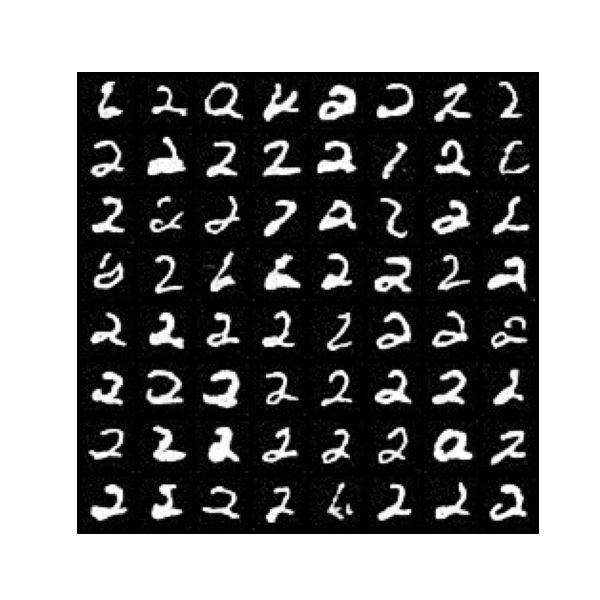
\includegraphics[width=\textwidth]{Chapters/figures/experiments/mnist/mnist_2.png}
    \end{subfigure}
    \begin{subfigure}{0.3\textwidth} \label{abb:1a}
        \centering
        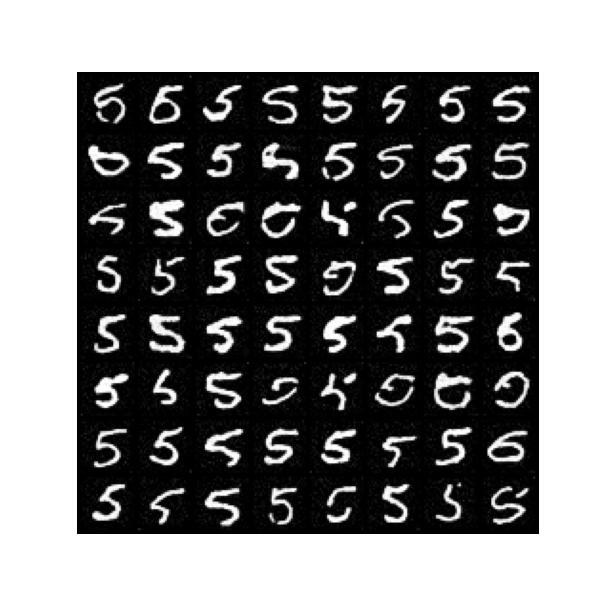
\includegraphics[width=\textwidth]{Chapters/figures/experiments/mnist/mnist_5.png}
    \end{subfigure}
    \begin{subfigure}{0.3\textwidth} \label{abb:1a}
        \centering
        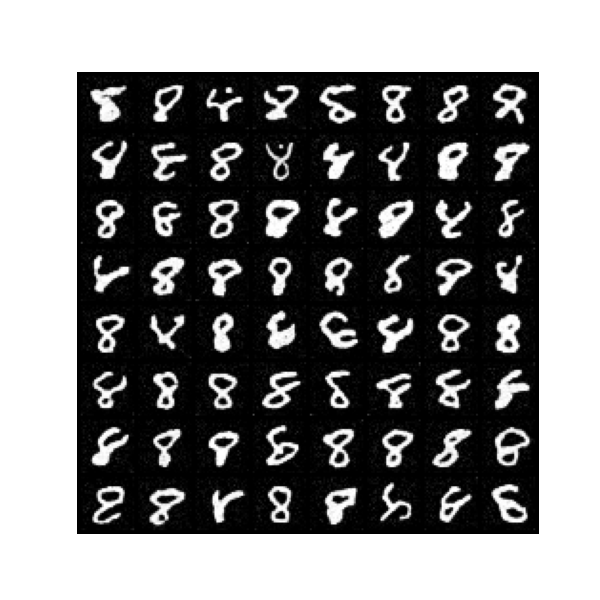
\includegraphics[width=\textwidth]{Chapters/figures/experiments/mnist/mnist_8.png}
    \end{subfigure}
    
    \caption{MNIST class-conditional results. \textit{Left:} 2, \textit{Middle:} 5, \textit{Right:} 8}
    \label{fig:my_label}
\end{figure}
%

%%%%%%%%%%%%%%%%%%%%%%%%%%%%%%%%%%%%%%%%%%%%%%%%%%%%%%%%%%%%%%%%%%%%%%%%%%%%%%%%%%%%%%%%%
\section{Semantic Synthesis Implementation} 
As described in \hyperref[sec:4.5]{Sec.\,4.5} a semantic segmentation network is needed to learn the forward process $\log p_t(\vec{y}|\vec{x}(t))$ which can be then used to solve the $\vec{y}$-dependent reverse SDE in \hyperref[equ:4.22]{Equ.\,4.22}. Effectively this means that the semantic segmentation is learned on noisy images $\vec{x(t)}$, where the noise for timestep $t$ is governed by the forward SDE. Since for each training image $\vec{x}(0)$ there also is a segmentation map $\vec{y}$, the guess $\tilde{\vec{y}}$ of the segmentation network can be compared to the true map to then compute an error. 

\subsection{Generating noisy training images}

As mentioned above – because the forward SDE is tractable – we can easily generate as much noisy training images as we want by adding noise to the initial training images $\{\vec{x}_i(0)\}_{i=1}^N$:
%
\begin{equation} \label{equ:5.1}
    \vec{x}(t)=\vec{x}(0)+\sigma(t)\cdot\vec{z}\,.
\end{equation}
%
In \hyperref[equ:5.1]{Equ.\,5.1} $\vec{z}\sim\mathcal{N}(0, \vec{I})$ is Gaussian noise and $\sigma(t)$ is the noise scale for timestep $t$ which for the VE SDE is given by
%
\begin{equation} \label{5.2}
    \sigma(t)=\sigma_{min}\cdot\left(\frac{\sigma_{max}}{\sigma_{min}}\right)^t.
\end{equation}
%
$\sigma_{min}$ corresponds to $\sigma(t=0)$ and is always chosen as $0.01$. Since the image information is in the range $[0,1]$, a noise of $0.01$ is not visible to the human eye. $\sigma_{max}$ corresponds to $\sigma(t=T\triangleq1)$ and is chosen as the maximum pairwise distance for the dataset under investigation. During training, for each not noisy training image in a batch we then randomly choose noise scales $\sigma(t)$ with $t\in[0,1]$ and transform the not noisy training batch into a noisy training batch by using \hyperref[equ:5.1]{Equ.\,5.1}.

\subsection{Choosing a noise encoding}

With the noisy images we can now train a semantic segmentation network. Obviously a semantic segmentation network is expected to perform increasingly worse on increasingly noisy images. To give an idea of the difficulty of the task, the maximum noise scale for the Cityscapes dataset is $338$, i.e. in images with maximum noise, the noise is $338$ higher than the underlying image information! Therefore, we cannot simply train a regular segmentation network $p_\theta(\vec{x(t)})$ on noisy images, but we need to condition the network on noise $p_\theta(\vec{x}(t), \sigma(t))$, so that it can better distinguish the noise scales. There are some advanced ways to encode this noise information, including \textit{Sinusoidal Positional Embeddings} \cite{attention} or \textit{Gaussian Fourier Embeddings} \cite{fourfeat}. These encoding techniques are used in NCSN++ to encode the noise information but for the segmentation network, we work with a much simpler type of encodings.

Our idea to condition the semantic segmentation is to encode the noise information as a $4th$ channel dimension in addition to the $3$ color channels for each pixel. The size of a batch of (noisy) training image has the size $N\times C\times H\times W$. We want to expand the noise information of size $N$ to size $N\times 1\times H\times W$ and than concatenate the noise with the images to obtain a resulting batch of size $N\times (C+1)\times H\times W$. This batch is then fed into the network.

However, there are several plausible options to express the noise of an image. The first option would be to use the noise scale itself, the second option would be to use the logarithm of the noise scale and the third option would be to use the timestep which directly correlates to noise. Recalling to the noise function in \hyperref[equ:5.2]{Equ.\,5.2} we can plot these three options in \hyperref[fig:5.2]{Fig.\,5.2}.

In order to evaluate these possibilities one needs to know the input format of the images into the network. Normally the pixel values are displayed in the range $[0, 1]$ rather than in the range $[0, 255]$. But since there is noise added to the initial images the pixel ranges can be everywhere from $[0,\sigma_{min}]$ and $[0, \sigma_{max}]$, depending on the current noise scale. When we tried to learn a segmentation network from images in various pixel ranges we got devastating results. Therefore we transform any perturbed image $\vec{x}(t)$ into the range $[0, 1]$ by using the following formula:
%
\begin{equation}
    \vec{x}_{[0,1]}(t)=\frac{\vec{x}(t)-\min(\vec{x}(t))}{\max(\vec{x}(t))-\min(\vec{x}(t))}.
\end{equation}
%

It is plausible that the noise encodings should be in a related order of magnitude than the image information. Therefore, we do not use noise scales as encodings because they are up to two magnitudes larger. Training one segmentation network conditioned on the logarithm of the noise scale $\log \sigma(t)$ and another conditioned on timesteps $t\in[0,1]$ revealed no significant differences. After 100 epochs on the cityscapes dataset we got a peak IoU (see TODO) of $\sim0.212$ for noise encodings and a peak IoU of $\sim0.213$ for timestep encodings. Since NCSN++ is conditioned on the logarithm of the noise scale, we also choose this encoding to condition our semantic segmentation network $p_\theta(\vec{x}(t), \log \sigma(t))$.

\subsection{Choosing a Semantic Segmentation Network}

There exists a wide variety of semantic segmentation networks that we could use. The problem with state-of-the-art segmentation networks is, that they often use pretrained classification networks in their architecture which makes them hard to condition on noise, because these pretrained networks are obviously not trained on noisy images. 

Therefore we first tried to use simpler models such as U-Net (\hyperref[sec:3.1.2]{Sec.\,3.1.2}) which are easy to implement and easy to condition on noise. The results we got were not really promising but it turned out that they actually were good enough to use them for semantic image synthesis. Concrete analyses of the trained segmentation networks in terms of pixel accuracy and IoU is presented in the dedicated experiment sections \hyperref[sec:5.4]{Sec.\,5.4}, \hyperref[sec:5.5]{Sec.\,5.5} and TODO.

We also tried to condition more complicated networks such as FCDenseNet \cite{densenet}, which significantly outperforms U-Net on non noisy images, but we could only achieve a peak IoU of $\sim0.146$ on noisy images, so we finally decided to use U-Net as semantic segmentation network for further experiments.

\subsection{Choosing an error function}

To compare the estimated semantic map $\tilde{\vec{y}}$ with the ground truth semantic map $\vec{y}$, we need to specify an error function. For U-Net the cross-entropy loss function is a good choice. Cross-entropy calculates the loss for an output given as probability value between $0$ and $1$ which is exactly what we (pixel-wise) have for a semantic segmentation network. The cross entropy operates on the logarithm of the output probability $\log p$. If the true label of a pixel is $1$ the loss is relatively low for probabilities $>0.2$ and grows rapidly for lower losses. For multiclass classification as for semantic segmentation the cross-entropy loss can be written as
%
\begin{equation}
    \Delta_{xy}=-\sum_{c=1}^C 
    \begin{cases}
        0, &\text{for } c\neq c_t\\
        \log p(c_t)_{xy}, &\text{otherwise}
    \end{cases}
\end{equation}
%
where $C$ is the total number of labels, $x$ and $y$ are the pixel-wise positions in the segmentation map, $c_t$ is the true label for position $xy$ and $p(c_t)_{xy}$ is the probability the network outputs for the pixel at position $xy$ having label $c_t$.
%
\subsection{Choosing a scale factor function}
As already touched upon in the previous section \hyperref[sec:5.1]{Sec.\,5.1} a scale factor for the gradients of the semantic segmentation network is necessary to obtain good sampling results. When using a static scale factor we observe that the pixel values often go into saturation, i.e. converging to $1$, which leads to overexposed samples. 

We are therefore interested in finding the time interval $T\subset[0,1]$ in which the gradients of the semantic segmentation network are the most needed, i.e. in which time interval important structural image information is formed and consolidated. With this information we hope to reduce the saturation effect on the final sample, because the semantic segmentation network is influencing the sample for a lower amount of time. We propose that for low noise ($t$ near $0$) the image structure is already consolidated and the semantic segmentation network only plays a minor role for generation. We further propose that for high noise ($t$ near $0$) the gradients of the segmentation network in theory would be beneficial for generation, but only if the network is capable to operate on high noise scales which we could not achieve up to maximum noise.

Therefore, as a scaling function we propose a function that is $0$ in regions where the network performs badly and $1$, in regions where the networks performs reasonable, followed by a linear decrease to $0$ for regions where we suggest that the image structure has already consolidated. To find out these regions we perform two experiments. In the first experiment we set the scale factor to $1$ for $t>t_{stop}$ and to $0$ for $t<=t_{stop}$, where $t_{stop}$ is subsequently reduced from $1$ to $0$ for each sample. In the second experiment we introduce $t_{start}$ for which for $t<t_{start}$ the scale factor is $1$ and for $t>=t_{start}$ the scale factor is $0$. The results – exemplary for one semantic map – can be seen in \hyperref[fig:5.4]{Fig.\,5.4} resp. \hyperref[fig:5.5]{Fig.\,5.5}.

Based on the findings for these experiments we generously conclude that for $t>0.8$ the segmentation network performs to badly to be helpful for generation and that for $t<0.4$ the structures in the image have already consolidated. We therefore propose the following scale function:
%
\begin{equation}
    s(t)=\begin{cases}
        0, &\text{for }t>0.8\\
        s_0, &\text{for }t<=0.8 \land t>0.4\\
        s_0-s_0\cdot(1-\nicefrac{t}{0.4}), &\text{for }t<=0.4
    \end{cases},
\end{equation}
%
where $s_0$ is the maximum scale factor for a given dataset, which is determined experimentally. The final gradients for sampling are therefore calculated via
%
\begin{equation}
    \nabla_{\vec{x}}\log p_t(\vec{x})+s(t)\cdot\nabla_{\vec{x}}\log p_t(\vec{y}|\vec{x}).
\end{equation}
%
\begin{figure} \label{fig:5.4}
    \tiny
    \centering
    \setlength\tabcolsep{-2pt}
    \begin{tabular}{cccc}
        Semantic map & Original image & T=0.8 & T=0.7 \\
        \includegraphics[width=0.25\textwidth]{Chapters/figures/experiments/seg_stop/0_1.0_seg_mask.png} &  \includegraphics[width=0.25\textwidth]{Chapters/figures/experiments/seg_stop/0_1.0_original.png} & 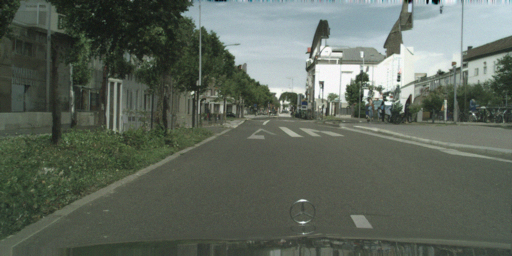
\includegraphics[width=0.25\textwidth]{Chapters/figures/experiments/seg_stop/0_0.8_cond_sample.png} & 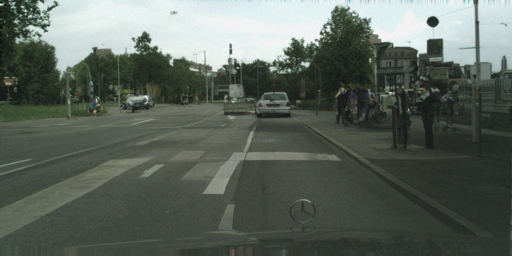
\includegraphics[width=0.25\textwidth]{Chapters/figures/experiments/seg_stop/0_0.7_cond_sample.png} \\
        T=0.65 & T=0.6 & T=0.55 & T=0.5\\
        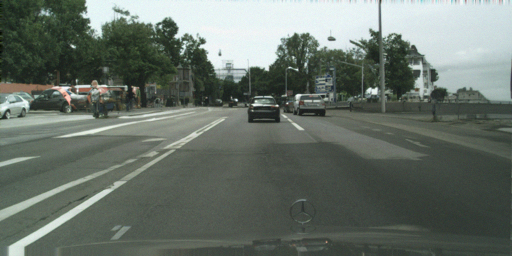
\includegraphics[width=0.25\textwidth]{Chapters/figures/experiments/seg_stop/0_0.6499999999999999_cond_sample.png} & 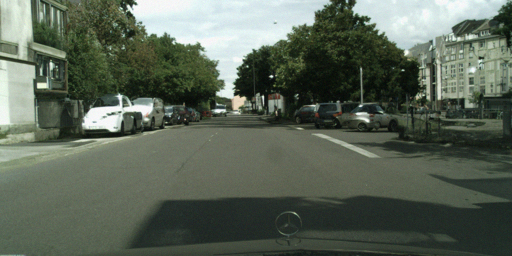
\includegraphics[width=0.25\textwidth]{Chapters/figures/experiments/seg_stop/0_0.6_cond_sample.png} & 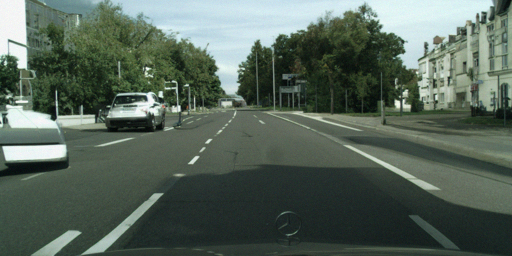
\includegraphics[width=0.25\textwidth]{Chapters/figures/experiments/seg_stop/0_0.55_cond_sample.png} & 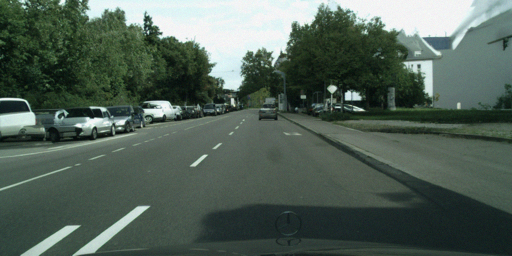
\includegraphics[width=0.25\textwidth]{Chapters/figures/experiments/seg_stop/0_0.5_cond_sample.png}\\
        T=0.45 & T=0.4 & T=0.2 & T=0\\
         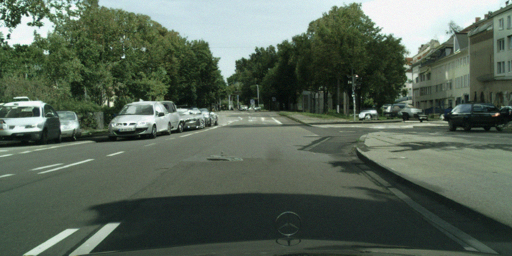
\includegraphics[width=0.25\textwidth]{Chapters/figures/experiments/seg_stop/0_0.44999999999999996_cond_sample.png} & 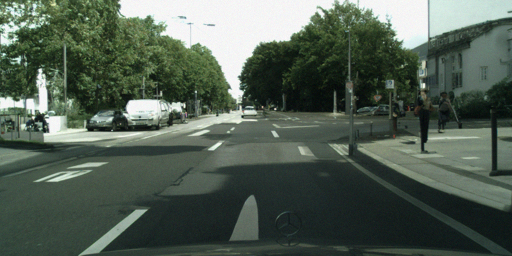
\includegraphics[width=0.25\textwidth]{Chapters/figures/experiments/seg_stop/0_0.3999999999999999_cond_sample.png} & 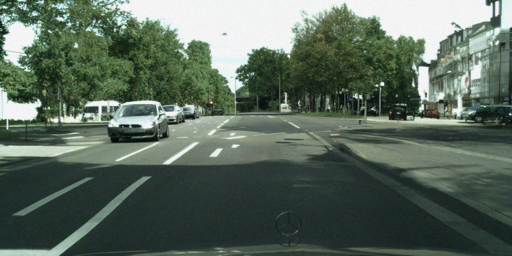
\includegraphics[width=0.25\textwidth]{Chapters/figures/experiments/seg_stop/0_0.19999999999999996_cond_sample.png}& 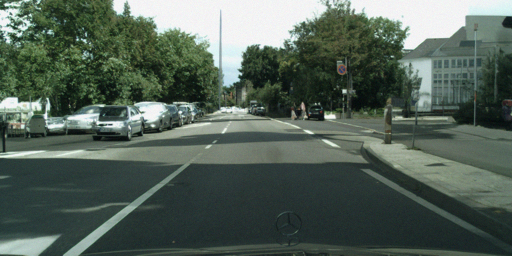
\includegraphics[width=0.25\textwidth]{Chapters/figures/experiments/seg_stop/0_0.0_cond_sample.png} 
    \end{tabular}
    \caption{Stop}
\end{figure}

\begin{figure} \label{fig:5.4}
    \tiny
    \centering
    \setlength\tabcolsep{-2pt}
    \begin{tabular}{cccc}
        Semantic map & Original image & T=0.2 & T=0.4  \\
        \includegraphics[width=0.25\textwidth]{Chapters/figures/experiments/seg_start/0_1.0_seg_mask.png} & 
        \includegraphics[width=0.25\textwidth]{Chapters/figures/experiments/seg_start/0_1.0_original.png} & 
        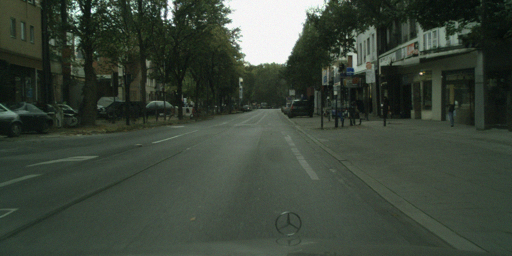
\includegraphics[width=0.25\textwidth]{Chapters/figures/experiments/seg_start/0_0.19999999999999996_cond_sample.png} & 
        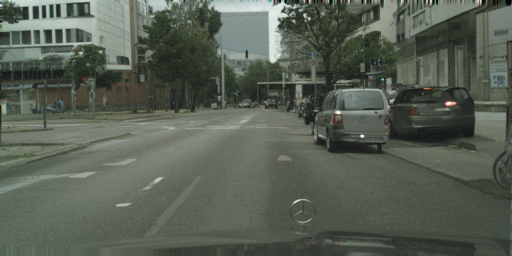
\includegraphics[width=0.25\textwidth]{Chapters/figures/experiments/seg_start/0_0.3999999999999999_cond_sample.png} \\
        T=0.5 & T=0.6 & T=0.65 & T=0.7  \\
        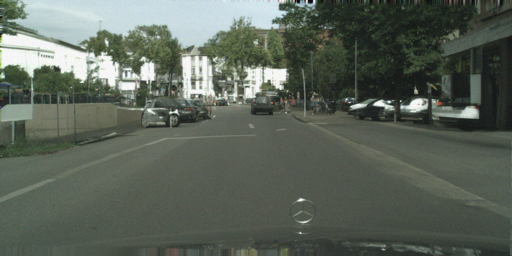
\includegraphics[width=0.25\textwidth]{Chapters/figures/experiments/seg_start/0_0.5_cond_sample.png} & 
        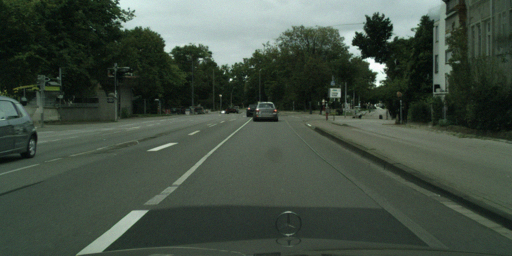
\includegraphics[width=0.25\textwidth]{Chapters/figures/experiments/seg_start/0_0.6_cond_sample.png} & 
        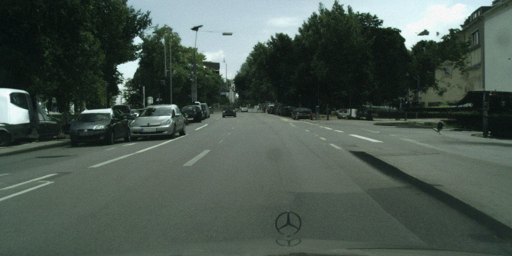
\includegraphics[width=0.25\textwidth]{Chapters/figures/experiments/seg_start/0_0.6499999999999999_cond_sample.png} &
        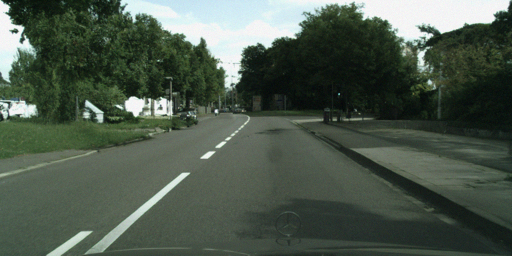
\includegraphics[width=0.25\textwidth]{Chapters/figures/experiments/seg_start/0_0.7_cond_sample.png}  \\
        T=0.75 & T=0.8 & T=0.9 & T=1  \\
        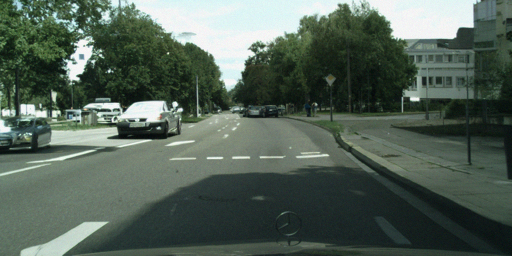
\includegraphics[width=0.25\textwidth]{Chapters/figures/experiments/seg_start/0_0.75_cond_sample.png} & 
        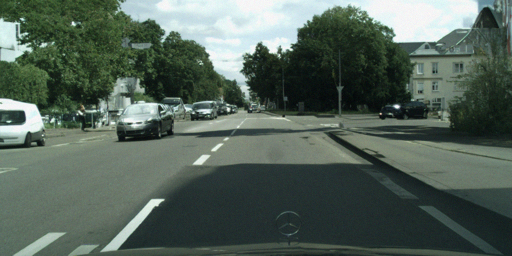
\includegraphics[width=0.25\textwidth]{Chapters/figures/experiments/seg_start/0_0.8_cond_sample.png} & 
        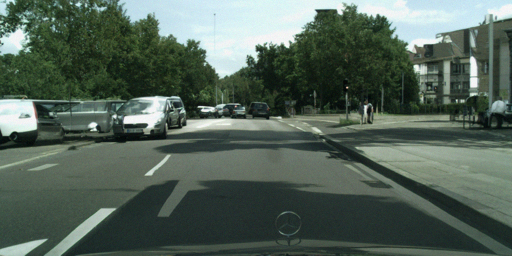
\includegraphics[width=0.25\textwidth]{Chapters/figures/experiments/seg_start/0_0.9_cond_sample.png} & 
        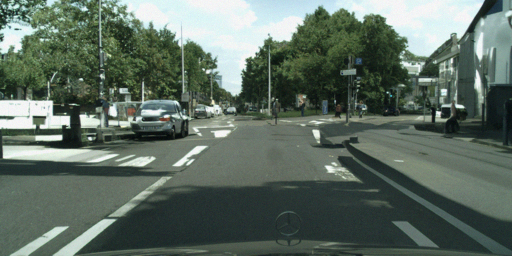
\includegraphics[width=0.25\textwidth]{Chapters/figures/experiments/seg_start/0_1.0_cond_sample.png}
    \end{tabular}
    \caption{Start}
\end{figure}
%%%%%%%%%%%%%%%%%%%%%%%%%%%%%%%%%%%%%%%%%%%%%%%%%%%%%%%%%%%%%%%%%%%%%%%%%%%%%%%%%%%%%%%%%%
\section{Improvements and Adaptations}
As initial experiments before testing semantic image synthesis on a large scale, we test the impact of two improvements/adaptations we made to the original score model architecture \cite{score_3}.
\subsection{Mixed precision learning} %0.5-1
vRAM usage and training speed are key aspects in training deep neural network. Complex models might consist of several million up to billion parameters to optimize. This requires an immense amount of computing power but at least equally important, vRAM. vRAM – video random access memory – is the memory that a GPU has available during operation. Modern high end consumer graphic cards typically have around $10GB$ of vRam. The crux of the matter is that reaching more than $10GB$ when training a moderately complex model is really easy and when training such complex models as NCSNs, the vRAM demand can increase beyond $100GB$, making training deep neural networks a very cost intensive business. Also when training complex models one can expect to need one week or more of training time, making testing and finetuning of models very exhausting.

To mitigate these problems the concept of \textit{Mixed Precision Learning} \cite{mixed_prec} was developed, decreasing both vRAM usage and training time with simultaneous retention of training quality, i.e. training loss. Normally each parameter of a network is stored as a float with $32bits$ of precision. Considering a network with $\sim250M$ parameters this would be equivalent to $\sim1GB$. What sounds not so much at first quickly becomes unmanageable when thinking of the series of matrix arithmetic's the parameters undergo and each calculation storing extra data such as gradients. 

The idea of mixed precision learning is to use floats with a $16bit$ precision wherever possible. In order to not loose model accuracy two concepts are applied. First, there is always a $32bit$ master copy of the model weights. For the forward pass this master copy is converted to $16bit$, where the complex gradient calculations happen. In the backward pass these $16bit$ gradients are converted back to $32bit$ where they are then used by the optimizer to update the master weights. But this improvement during gradient calculation comes with the flaw of loosing some gradients as every number $<2^{-24}$ is equal to $0$ for $16bit$ precision but in most models there is at least some relevant gradient information in the range $[2^{-27},2^{-24})$. To mitigate this effect the concept of loss scaling was proposed. Loss scaling multiplies the $32bit$ loss after the forward pass by a scale factor to move them in the $16bit$ range in which the gradients are then computed in the backward pass. Thereafter the scaled $16bit$ gradients are converted to scaled $32bit$ gradients and then divided by the same scale factor as before. Finally these scaled gradients are used by the optimizer to update the master weights. The full concept can be seen in \hyperref[fig:3.2]{Fig. 3.2}.
%
\begin{figure}[] \label{fig:3.2}
    \centering
    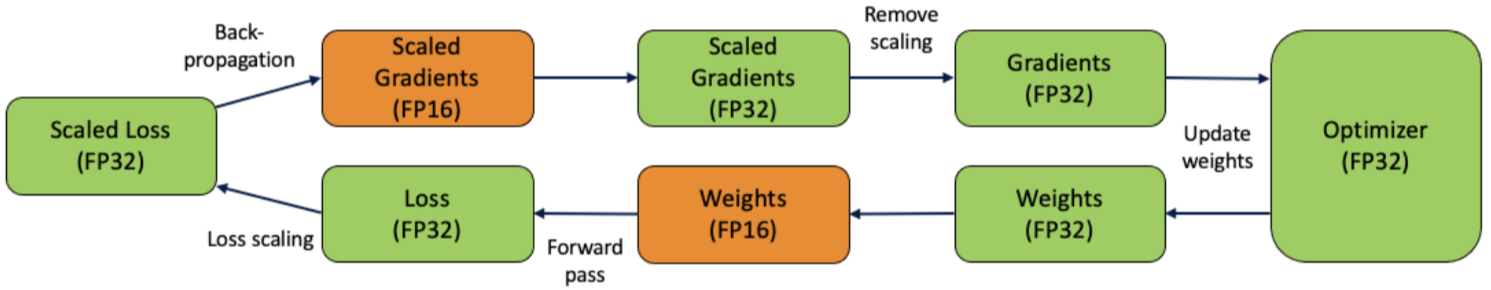
\includegraphics[width=.9\textwidth]{Chapters/figures/mixed_prec.PNG}
    \caption[Short-form caption]{Concept of Mixed Precision}
\end{figure}
%

As the mixed precision technique was not used in the original SGM paper \cite{score_3} it was now implemented using the off the shelf pyTorch tools for mixed precision to check how much this technique improves vRAM usage and training time for the NCSN. To do so we trained the NCSN++ on the Cityscapes dataset on two different GPUs with the same model settings. For each GPU $2\times100$ epochs were passed, once with mixed precision on and once with mixed precision off. The first GPU was a \textit{Nvidia GeForce RTX 2080 Ti} with $11GB$ of vRAM and the second GPU was a \textit{Nvidia A100} with $40GB$ of vRAM. For both GPUs we used the maximum possible batch size for non mixed precision training which is $1$ for the RTX 2080 Ti and $5$ for the A100. The effects of mixed precision training on vRAM usage and training time can be seen in \hyperref[tab:3.1]{Tab. 3.1} resp. \hyperref[tab:3.1]{Tab. 3.2}. For the vRAM usage the total vRAM needed is shown and for the training time the average training time for one epoch is shown.
%
\begin{table}[] \label{tab:3.1}
        \centering
    \begin{tabular}{c|c|c}
        GPU type        & Mixed precision \textbf{Off}    & Mixed precision \textbf{On} \\
        \hline
        RTX 2080 Ti     &  7791MB               & 7367MB\\
        A100            &  39039MB              & 29481MB
    \end{tabular}
    \caption{vRAM usage w/ and w/o mixed precision}
\end{table}
\begin{table}[b] \label{tab:3.2}
        \centering
    \begin{tabular}{c|c|c}
        GPU type        & Mixed precision \textbf{Off}    & Mixed precision \textbf{On} \\
        \hline
        RTX 2080 Ti     &  1494s                & 1206s    \\
        A100            &  965s                 & 987s
    \end{tabular}
    \caption{Training time per epoch w/ and w/o mixed precision}
\end{table}

For the A100 serious improvements on vRAM usage can be observed. For the RTX 2080 Ti there are only little improvements for vRAM usage but good improvements on training time. In general mixed precision is expected to perform way better on the new Ampere GPU
architecture (A100) than on the older Turing GPU architecture (RTX 2080 Ti). To ensure that the training quality does not suffer from the use of mixed precision the loss curves for all test setups are compared in \hyperref[fig:3.3]{Fig. 3.3}. The higher fluctuations for the RTX 2080 Ti are due to the fact that the batch size is smaller, therefore leading to major loss differences in a batch-to-batch comparison. In general it can be seen that mixed precision has no notable effect on training loss. Also a qualitative comparison of generated samples shows no difference perceptible by a human. We therefore conclude that – at least for non FID record breaking attempts – mixed precision should be used and we do so for all upcoming experiments.
%
\begin{figure} \label{fig:3.3}
    \centering
    \begin{subfigure}[b]{0.49\textwidth}
        \centering
         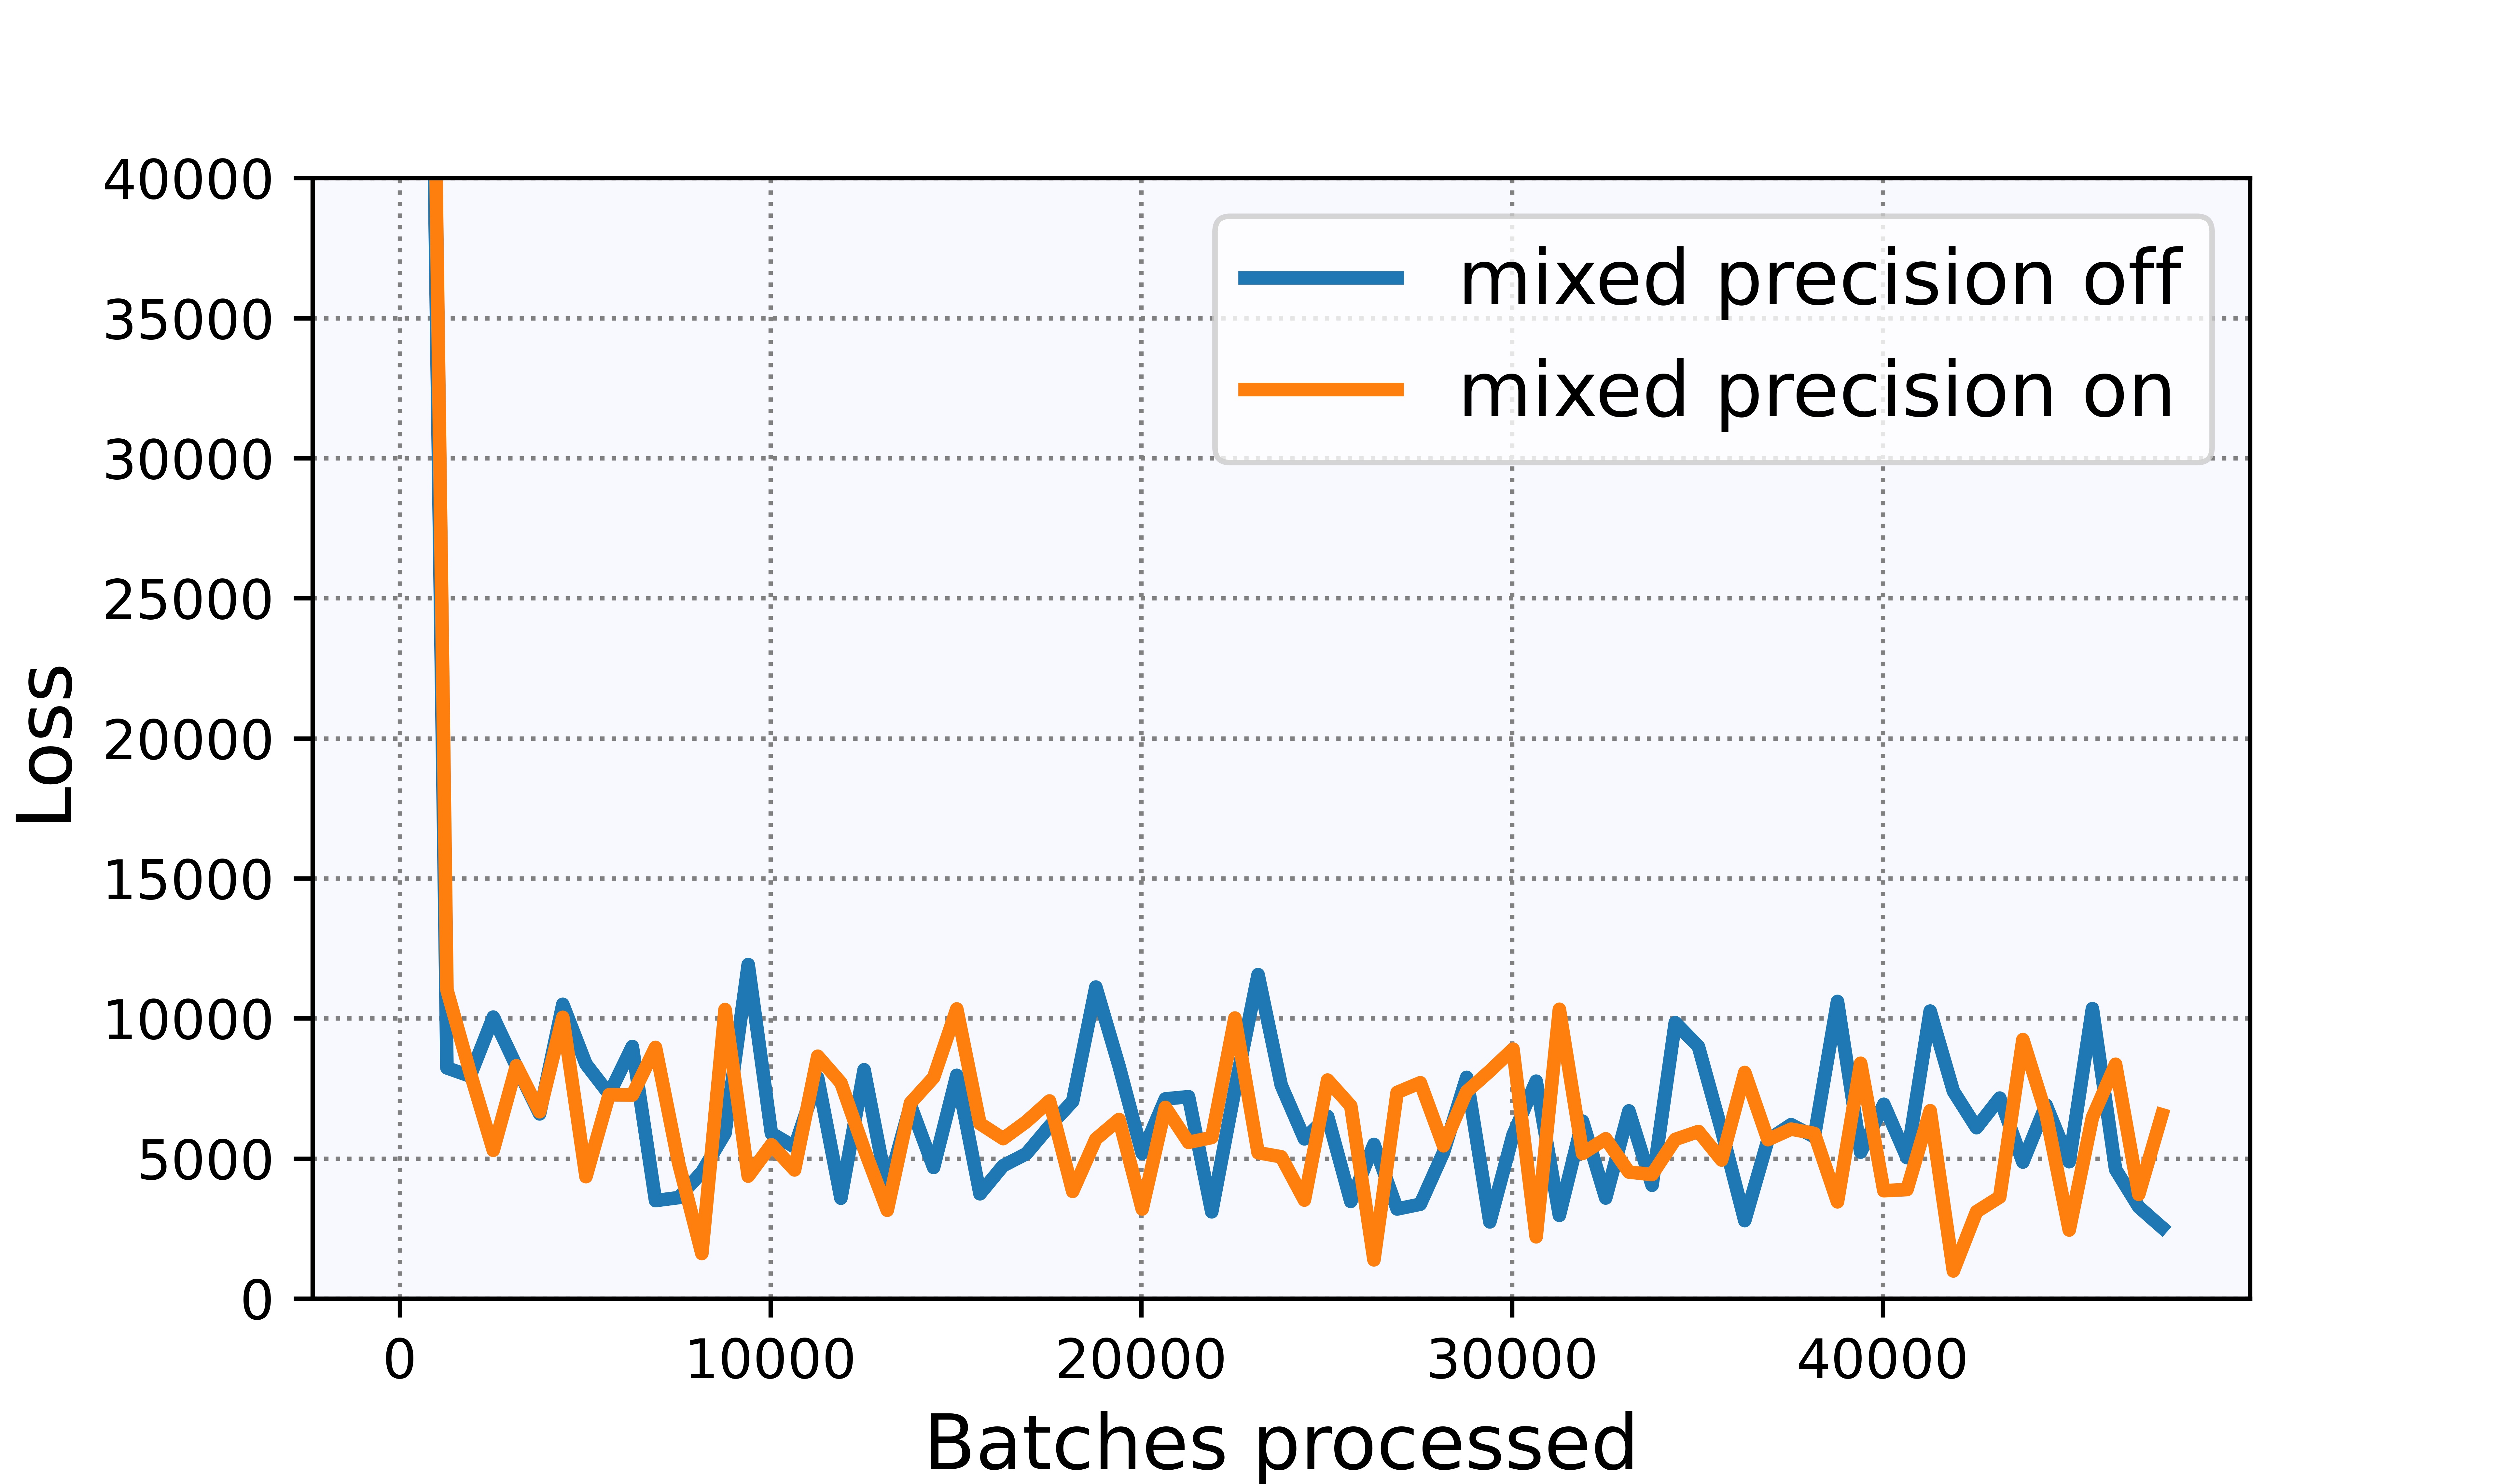
\includegraphics[width=\textwidth]{Chapters/figures/mixed_prec_rtx2080_loss.jpg}
         \caption{Loss curve RTX 2080 Ti}
    \end{subfigure}
    \begin{subfigure}[b]{0.49\textwidth}
        \centering
         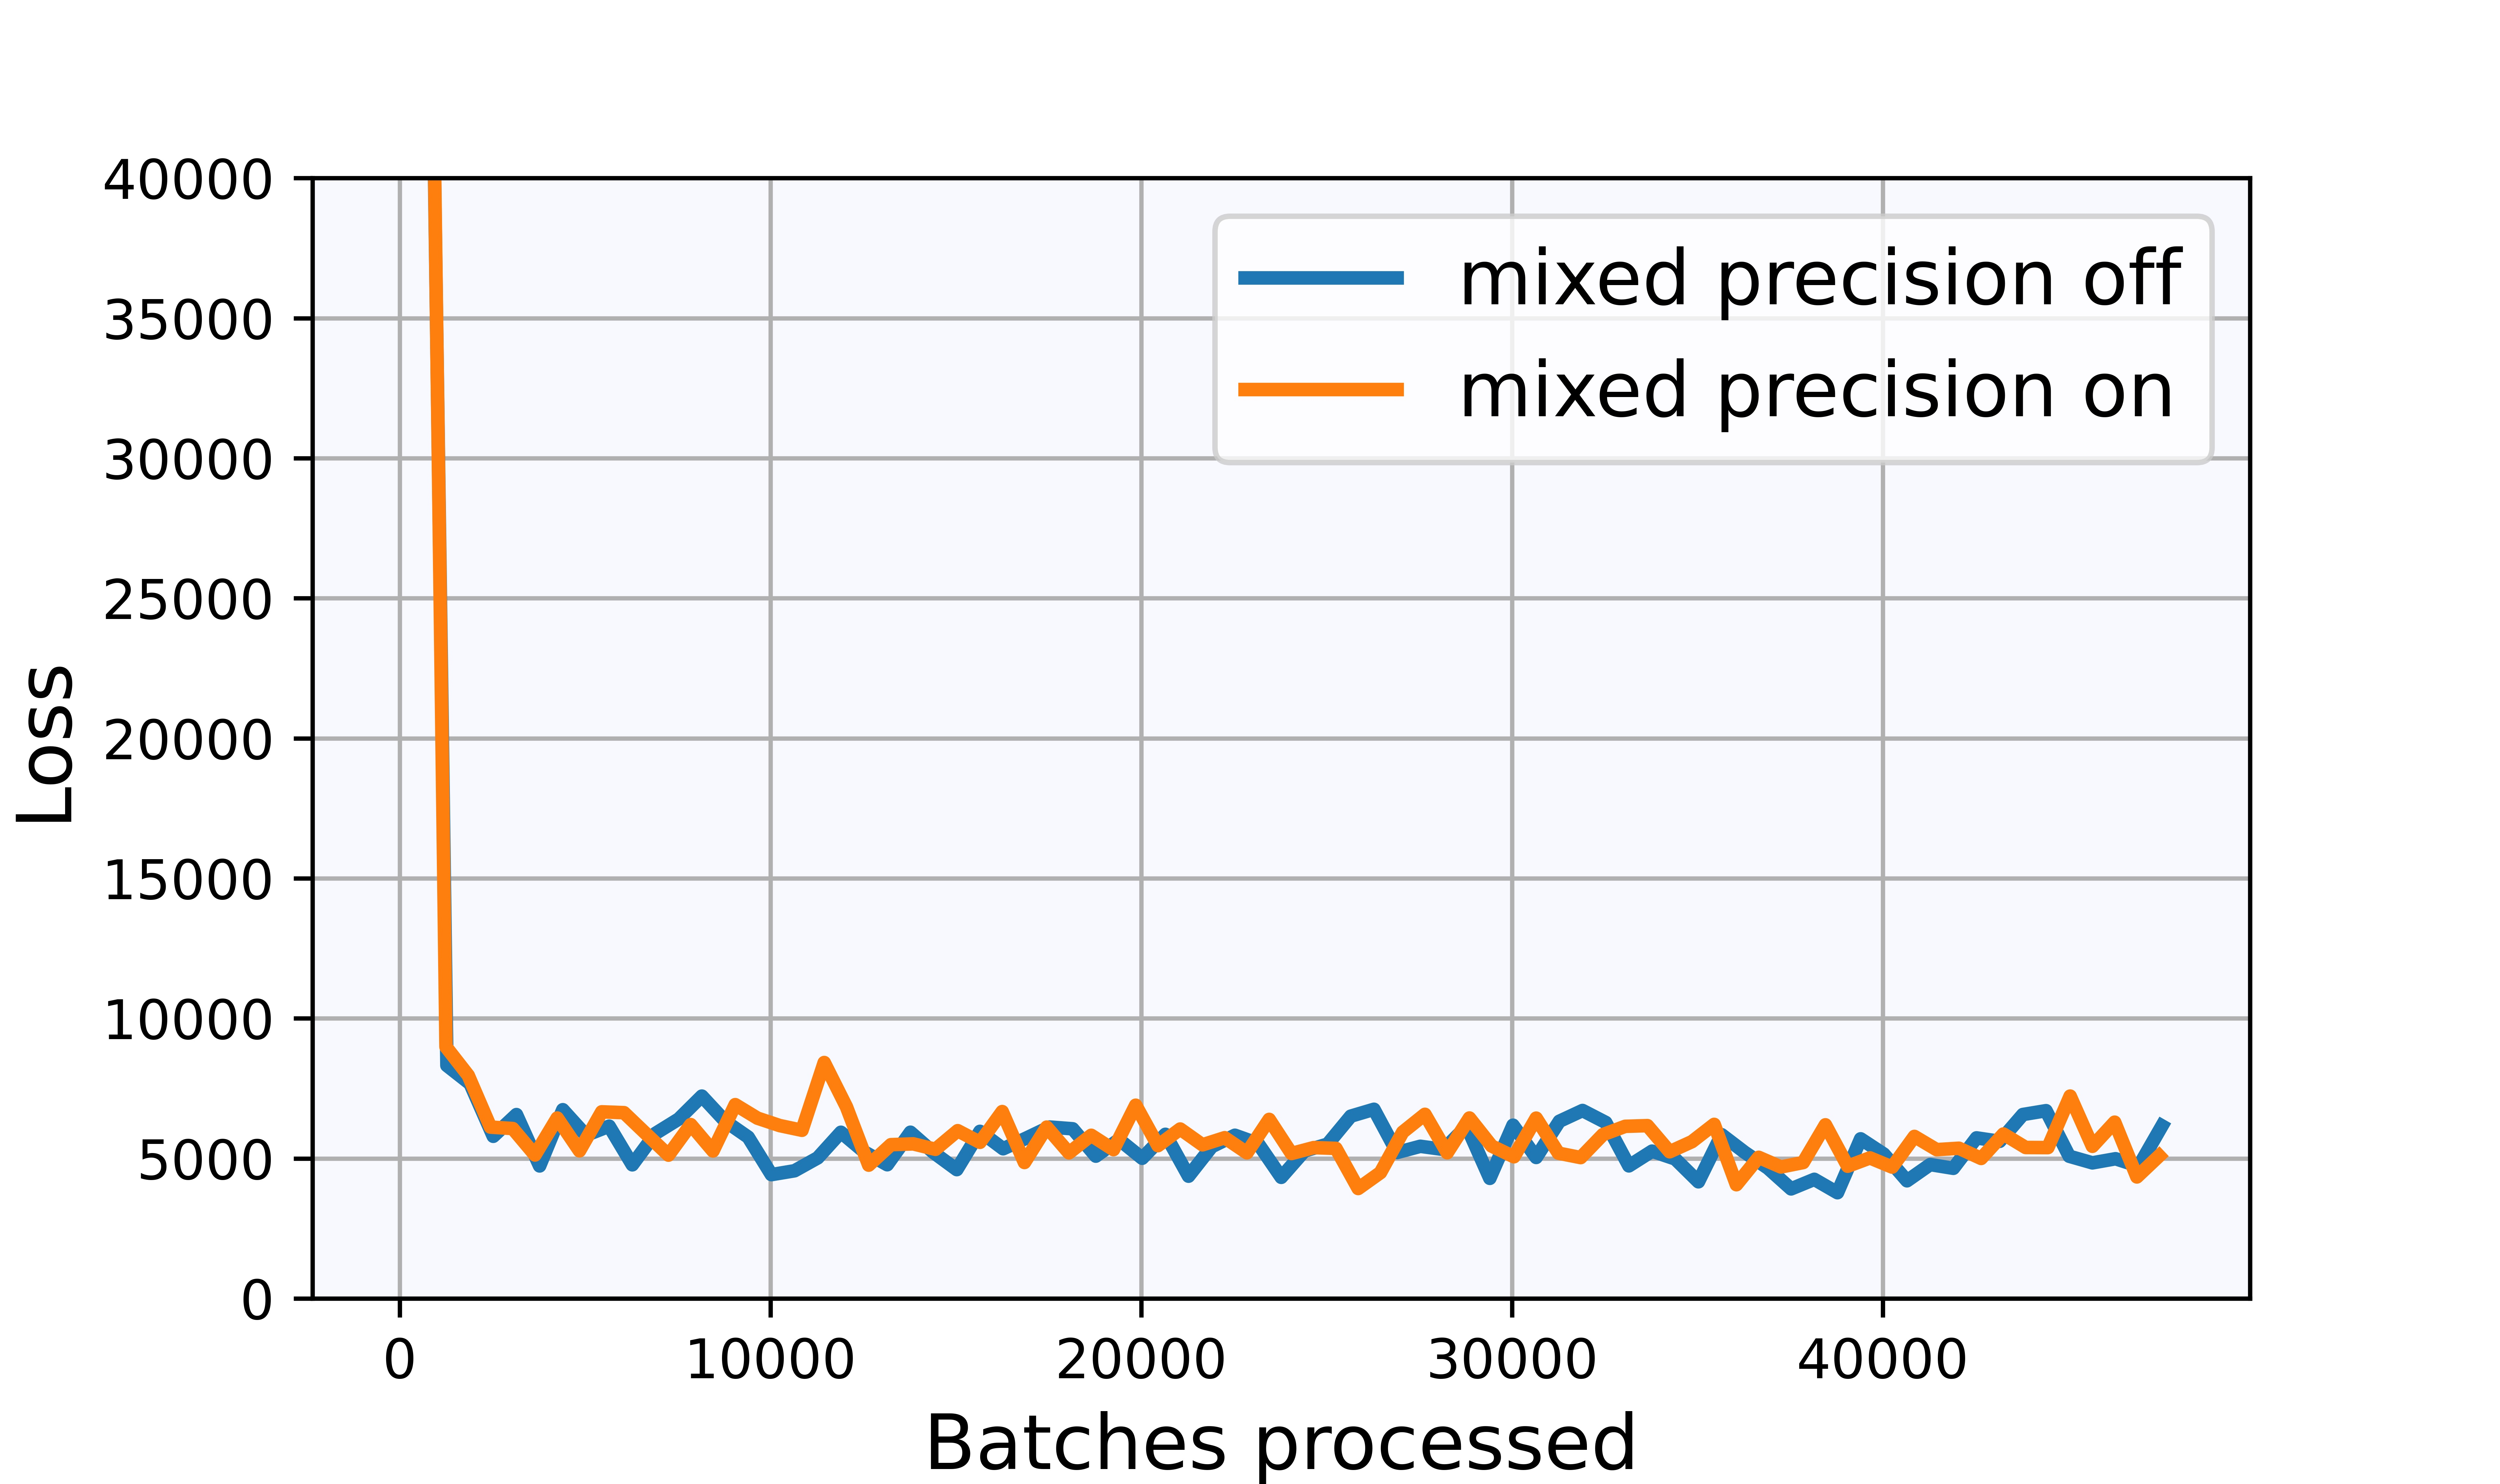
\includegraphics[width=\textwidth]{Chapters/figures/mixed_prec_a100_loss.jpg}
         \caption{Loss curve A100}
    \end{subfigure}
    \caption{Comparing loss curves for mixed precision \textbf{on} an \textbf{off} for both GPUs}
\end{figure}
%
\subsection{Training on arbitrary image sizes} %0.5-1
When training a generative model the image size the model gets as input for learning can have a large effect on what the model learns. Here not the total image size of the images is meant but the image size the model gets as input. As an example the cityscapes dataset (downscaled) consists of $256\times512$ pixel images. To reduce vRAM during training, the images from the dataset often are randomly cropped to another resolution, here $256\times256$. For some datasets this has only little negative effects on the model accuracy, e.g. for landscapes where the relative position of objects to each other only plays a minor role. But for datasets as the cityscapes dataset it is quite important for realistic results that the models learns the logic of images showing street scenes, i.e. learning that the street is in the middle, that there are parking cars on the left and right side of the image and so on. Training on too small crops can hinder the model to learn such logic.

As the version of NCSN \cite{score_3} does not support training on/sampling of non-square images, the model was adapted to do so. Actually the model already was able to process non-square images natively but there was a small bug that we fixed to make non-square training/sampling possible. To show the importance of this bugfix we investigate the influence of the above described effect on NCSN. For this purpose we trained two identical NCSN, one on $256\times256$ crops and one on the $256\times512$ original images. Some example results can be seen in \hyperref[tab:5.3]{Tab.\,5.3}. It is clearly visible that the full image model outperforms the cropped image model when the focus of evaluation is on street scene logic. It must be mentioned that for semantic image synthesis – the task for our experiments – this logic information actually is given by the semantic map which initially gives rise to the idea of training on crops at all. Nevertheless we suspect that a model knowing the logic without a semantic map also performs somewhat better than if it did not. For that reason models for further experiments on the cityscapes dataset were always trained with the full size images.
\begin{table}[] \label{tab:5.3}
    \centering
    \setlength\tabcolsep{-2pt}
    \begin{tabular}{ccc}
        & Training size $256\times256$ & \\
        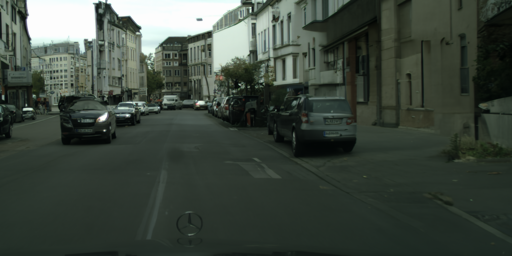
\includegraphics[width=0.33\textwidth]{Chapters/figures/experiments/crop/1_sample.png} &
        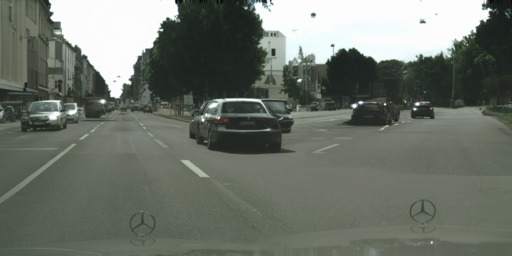
\includegraphics[width=0.33\textwidth]{Chapters/figures/experiments/crop/5_sample.png} &
        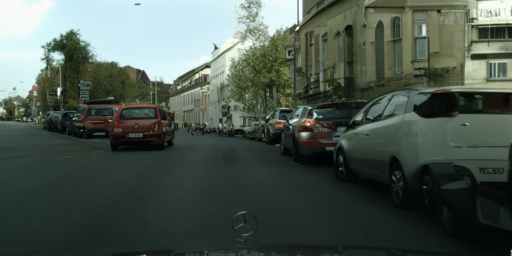
\includegraphics[width=0.33\textwidth]{Chapters/figures/experiments/crop/8_sample.png}\\
        & Training size $512\times256$ & \\ 
        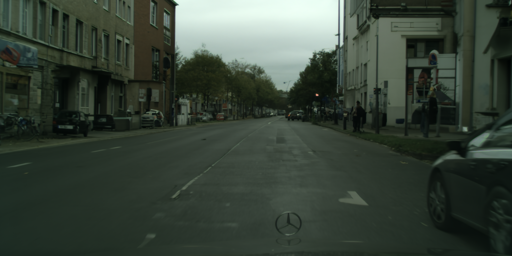
\includegraphics[width=0.33\textwidth]{Chapters/figures/experiments/crop/0_uncond_sample.png} &
        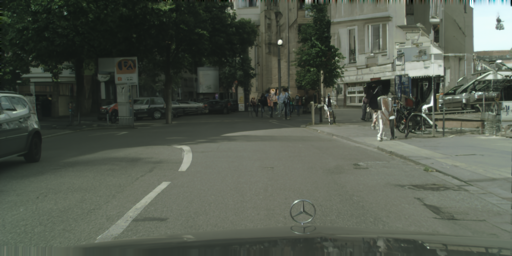
\includegraphics[width=0.33\textwidth]{Chapters/figures/experiments/crop/3_uncond_sample.png} &
        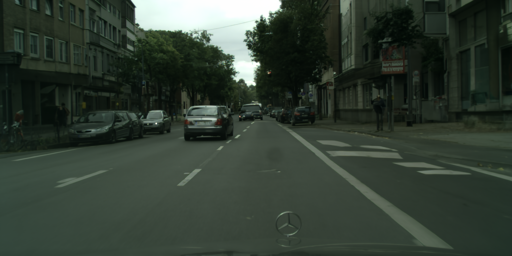
\includegraphics[width=0.33\textwidth]{Chapters/figures/experiments/crop/7_uncond_sample.png}
    \end{tabular}
    \caption{Unconditional example images of NCSN trained on cropped images (\textit{top}) and full size images (\textit{bottom}).}
    \label{tab:my_label}
\end{table}

%%%%%%%%%%%%%%%%%%%%%%%%%%%%%%%%%%%%%%%%%%%%%%%%%%%%%%%%%%%%%%%%%%%%%%%%%%%%%%%%%%%%%%%%%%%%%%%%%

\section{A competitive experiment on the Cityscapes dataset} \label{sec:5.4}

\subsection{The Cityscapes dataset}
\subsection{Metrics}

\section{Synthesizing high resolution landscapes} \label{sec:5.5}





\chapter{Conclusions and outlook} %2-3
%min 32 max 47
\appendix 
\chapter{Lists}
\listoffigures
\listoftables

\listofalgorithms

\bibliography{bibliography}
%\addcontentsline{toc}{chapter}{Bibliography}

\chapter{Deposition}
Ich versichere, dass ich diese Arbeit selbstst\"{a}ndig verfasst und keine anderen als die angegebenen Quellen und Hilfsmittel benutzt habe.
\\\\
\noindent I hereby assure that I have written this thesis independently and that I have not used any sources or aids other than those indicated.
\\\\
\noindent Heidelberg, den 19. Juli 2021
\\\\
\noindent Heidelberg, July 19, 2021
\\\\

\includegraphics[width=.5\textwidth]{Chapters/figures/unterschrift.PNG}


\end{document}
